\documentclass[11pt]{acmeArticle}
\usepackage{amssymb,amsthm,mathrsfs,graphicx}
\usepackage{natbib}
\usepackage{subfigure}
\usepackage{titlesec}
\usepackage{geometry}
\usepackage{fancyhdr}
\usepackage{newtxtext,newtxmath}
\usepackage{hyperref}

\usepackage{amsmath}
\usepackage{color}
\usepackage{amsfonts}
%\DeclareMathOperator*{\Aoperator}{ \mathlarger{\mathlarger{\mathlarger{\boldsymbol{\mathsf{A}}}}} }
\DeclareMathOperator*{\aoperator}{ \text{\huge${\rm{A}}$}}
\pagenumbering{arabic}


\setlength{\parindent}{0pt}
\setlength{\parskip}{5pt plus 2pt minus 1 pt}

\numberwithin{equation}{section}
%\topmargin  -25mm
%\evensidemargin 0mm
%\oddsidemargin  0mm
%\textwidth  160mm
%\textheight 267mm
\renewcommand{\baselinestretch}{1.0}
\frenchspacing
\sloppy
\titlespacing{\section}{0pt}{\parskip}{0.01\parskip}
\renewcommand{\headrulewidth}{0pt}
%%%%%%%%%%%%%%%%%%%%%%%%%%%%%%%%%%%%%%%%%%%%%%%%%%%%%%%%%%%%%%%%%%%%%%%


\begin {document}
\vspace*{-1mm}
\thispagestyle{fancy} 
%\fancyhead[R]{{}
\rhead{{\footnotesize
		\it September 2018, Glasgow\\} }
\cfoot{}

\pagestyle{empty}

\begin{center}
	
	{\fontsize{14}{20}\bf Strain release energy in remodelled equine metacarpal bone - numerical investigation.}\end{center}

%\restoregeometry

\begin{center}
	\textbf{Karol Lewandowski }\\
	\textbf{{\L}ukasz Kaczmarczyk, Ignatios Athanasiadis, John F. Marshall, Chris J. Pearce }\\
	{School of Engineering} \\
	{University of Glasgow}
\end{center}
%
{\clearpage}

\begin{center}
	\textbf{ABSTRACT}\\[1mm]
\end{center}
%


{\small 
	Fractures of the metacarpal condyle are a common orthopaedic injury in Thoroughbred racehorses.  
	A large proportion of injuries occur in the absence of a specific traumatic event and show typical characteristics of stress fractures. 
	The purpose of this work is to develop a combined remodelling and fracture finite element based framework allowing for integrated simulation of an~equine 3rd metacarpal remodelling under specific exercise regime (boundary conditions), followed by the evaluation of its fracture release energy. 
	The proposed approach can improve the understanding of the correlation between high intense exercise intensity, bone adaptation and fracture 
	risk, ultimately improving the welfare of the racehorse. 
	The remodelling analysis is based on a phenomenological model of the macroscopic behaviour of bone based on thermodynamics of open 
	systems previously presented in the literature. 
	Assessment of fracture propensity is conducted by evaluating strain release energy rate within the context of configurational mechanics. 
	All analyses are performed using unstructured tetrahedral meshes. 
	Material mapping between remodelling analysis mesh and fracture analysis mesh is obtained through Moving Least Squares approximation. 
	Hierarchical basis functions of arbitrary polynomial order are adopted to increase the order of approximation to achieve high 
	accuracy results with relatively coarse meshes and to take advantage of efficient multigrid solvers.
	Extension of Quarter Point Elements tailored for hierarchical basis functions is proposed to solve the stress singularity at the 
	crack tip.
	The implemented framework provides a robust and energy consistent method for quantifying the influence of bone adaptation on the
	 fracture propensity
	Performance, verification, convergence and validation of the presented method are demonstrated by numerical examples.
	The promising results of this study offer a~novel framework to simulate changes in the bone structure in response to exercise and 
	quantify the fracture propensity.
	 
	%Bone is able to adapt to changes in its mechanical environment. Studies of the Thoroughbred racehorse show modification of the geometric properties of the third metacarpal bone in response to training. These modifications are associated with reduced bone strains. Intense training before the adaptive response is completed and bone strain reduced increases the risk of fatigue damage. Bone adaptation in response to different loads is known to increase the resistance to fracture. The development of computational models to describe bone behavior has gained tremendous importance over the last decade. In particular, computational modelling for bone growth and resorption processes followed by fracture analysis can be a useful tool to determine crack propensity. Therefore,, this study aims to develop an efficient framework which will help to understand the relationship between exercise loading, bone density and ultimately fracture risk. This case study highlights the development of subject-specific FE analyses to simulate exercise loading on equine bone and subsequently quantify changes in the fracture propensity in open source code - MoFEM.
	
\textbf{\textit{Key Words:}} {\it finite element analysis, bone remodelling, fracture, 3rd metacarpal, moving least squares, configurational mechanics, heterogeneity}}
%
\\
\newpage

\textcolor{red}{All the figures are still in draft mode.}
\section{Introduction}
Fractures of the third metacarpal bone are one of the main reasons for euthanasia of Thoroughbred racehorses on racecourses in the UK \citep{Parkin2004risk}.
Most of these fractures occur due to the accumulation of tissue fatigue as a result of repetitive loading \citep{Parkin2005} rather than specific traumatic event.
Remodelling is the on-going complex biological process of replacing old bone tissue by new bone and thus repairing the fatigue damage\citep{hughes2017role}.
However, the racehorse is an extreme example of this process in which intense exercise and excessive loading of the metacarpal bones results in maladaptation.
The bone repair is overwhelmed by load-induced bone densification that also increases brittleness \citep{loughridge2017qualitative}.
The location of 3rd metacarpal fractures is remarkably consistent as a large number of racehorses present crack initiation from 
the lateral lateral para-sagittal groove of the distal condyle of the leading forelimb \citep{jacklin2012frequency, parkin2006analysis}.
However, despite a considerable research in the field, including applying diagnostics methods like radiography 
\citep{bogers2016quantitative, crijns2014intramodality, loughridge2017qualitative}, magnetic resonance imaging 
\citep{tranquille2017MRI} or biomarkers \citep{mcilwraith2005use}, it still remains a challenge to accurately predict the fracture risk 
and prevent this type of significant injury.
Therefore, development of computational tools with the capability to estimate bone adaptation and its resistance to fracture is a potential 
viable and robust solution.
The use of numerical models to describe bone behaviour has gained a tremendous importance over the last decade. 
In particular, Finite Element Method has been used to improve understanding of the fracture behaviour of bones and the relationships between load conditions and bone architecture \citep{podshivalov2014road, poelert2013patient}. \\
The goals of this study are to explore the potential of a computational framework based on FEM to predict bone density profiles 
(bone adaptation) for the undergoing exercise (training) and subsequently quantify fracture resistance of 
adapted bones using linear fracture mechanics for brittle materials. 
A schematic of the procedure is presented in Figure \ref{fig:framework}.
%(The aim for this study is the establishment and implementation of FEM based framework suitable for clinical practice that will help to simulate density evolution, quantify current and future fracture risk based on CT scanning data derived from horses in training.) 
Bone adaptation process, within the developed framework, is incorporated by using computational algorithm in open system thermodynamics 
\citep{Kuhl2003a}.

The rest of the article is structured as follows.
A brief review of open system thermodynamics is presented in Section \ref{sec:bone_remodel}.
Moreover, a novel approach to assign heterogeneous mechanical bone properties, derived from CT scans,
to the FE model by means of the Moving Least Squares (MLS) method is proposed in Section \ref{sec:dens_mapping}.
Examples and verification of the proposed approach are also demonstrated. 
Thereafter, Section \ref{sec:release_energy} encompasses extension of recently established energy consistent approach 
for evolving crack propagation in the context of configurational mechanics. 
The method is utilised to calculate release energy of bones under quasi-static loading during different stages of adaptation. 
Section \ref{sec:numerical_examples} brings together all the developments of the framework in the form of numerical examples. 
Finally, in Section \ref{sec:discussion} a brief summary of the work is presented and areas for further research are identified.
\begin{figure}[h!]
\begin{center}
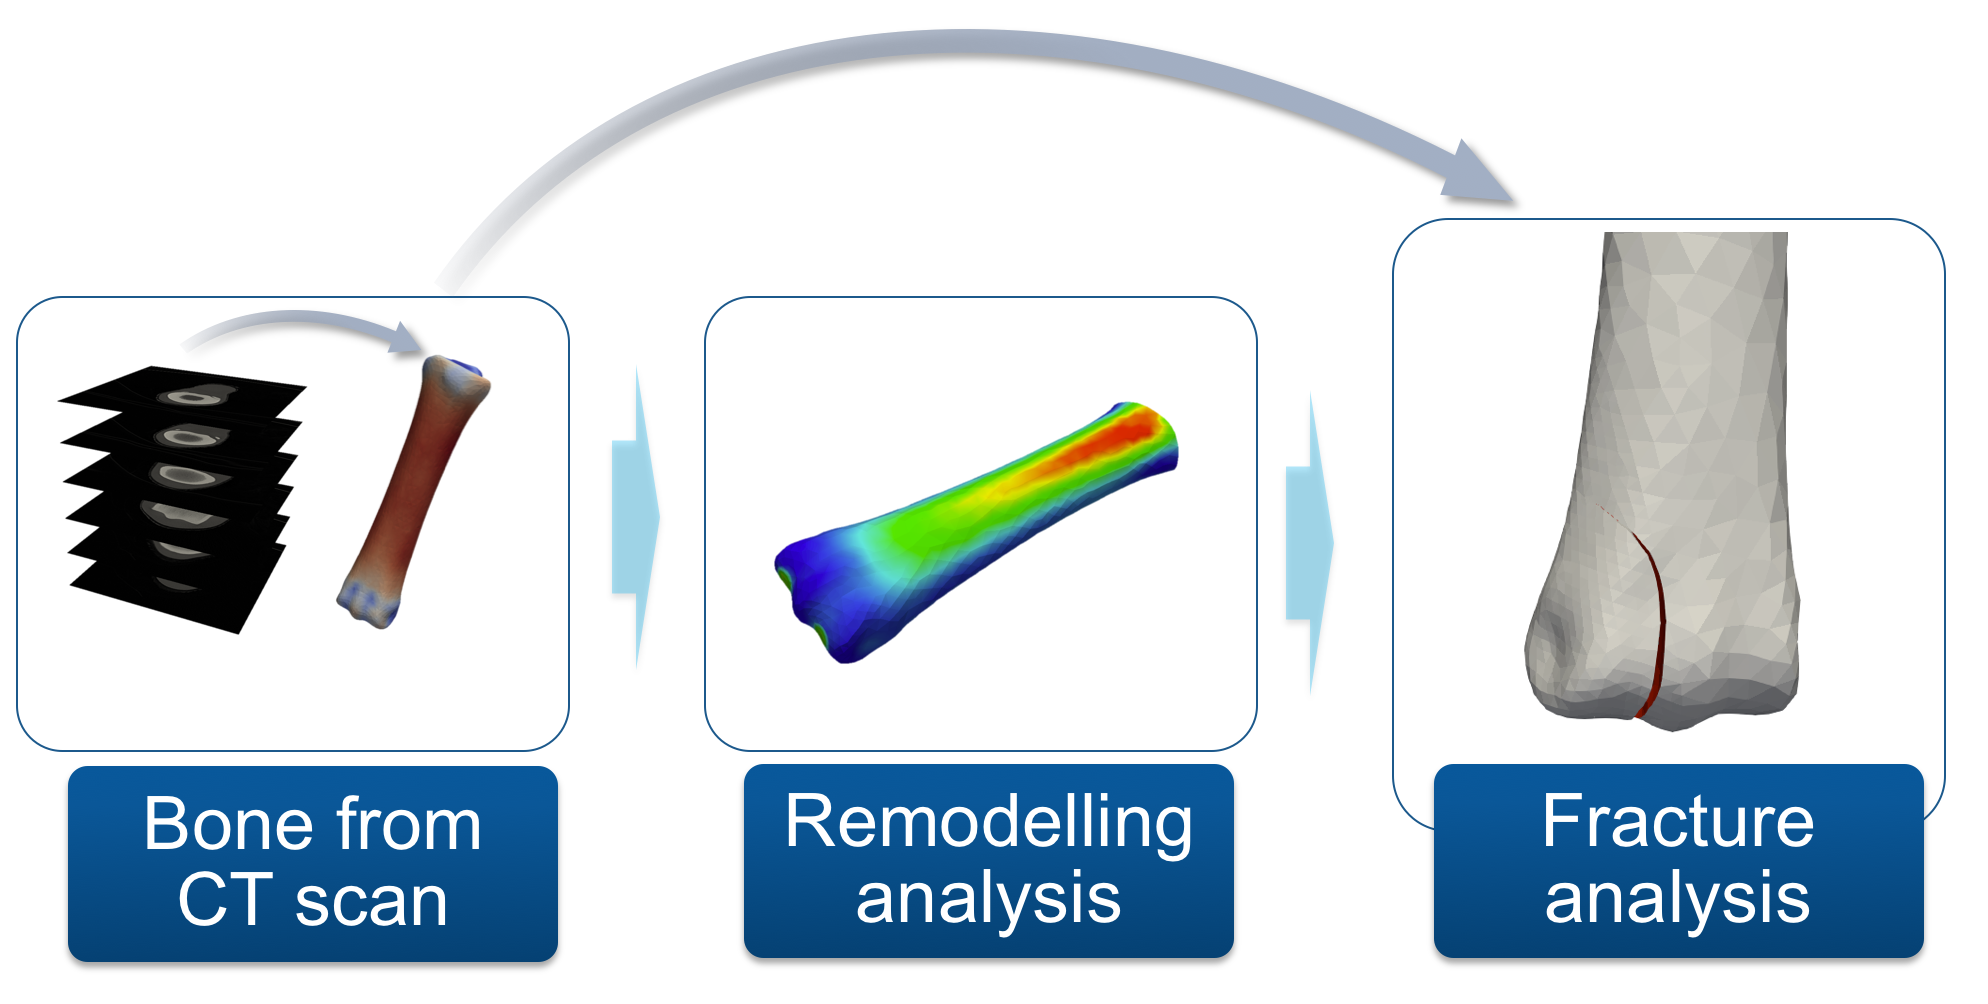
\includegraphics[width=12cm,height=12cm]{Figures/framework.png}
\caption{Framework for estimating crack propensity in MoFEM \citep{mofem2017}. Density derived from Quantitative Computed Tomography (qCT) is mapped onto finite element mesh, which is subsequently used for bone remodelling analysis. Next, utilizing the fracture mechanics module the released energy of an initial crack is computed at different time steps.}
\label{fig:scales}
\end{center}
\end{figure}

\section{Bone remodelling} 
\label{sec:bone_remodel}
Stress fractures are strongly correlated with the remodelling process \citep{hughes2017role}. 
The bone's ability to repair micro-damage caused by cyclical loading is essential for maintaining the mechanical integrity. 
One of the first mathematical theories for bone remodelling, based on open system thermodynamics has foundations in the 
theory of poroelasticity \citep{cowin1976bone}. 
Since it was introduced in the 1970s, it has become a popular area of interest within the field of modelling biomechanical processes. 
In this theory, unlike in classical closed systems, energy, mass, momentum and entropy can cross the boundary of the body and 
be exchanged with its environment. 
Many derivations and enhancements of this approach have been developed over the years. 
For example, researchers were able to capture the functional adaptation of the bones by means of optimisation theory
 \citep{harrigan1996bone, jacobs1995numerical, weinans1992behavior}.
%explain this better
The general concept for density evolution within these approaches is to establish a~mechanical stimuli as triggers for bone adaptation. 
The stimulus may take the form of stress \citep{beaupre1990approach, carter1996mechanical, doblare2002anisotropic}, strains \citep{cowin1976bone} or strain energy density \citep{weinans1992behavior, kuhl2003theory,kaczmarczyk2011efficient, Connor2017bone}. 
\\ 
In this contribution functional adaptation of the equine 3rd metacarpal bone is modelled by using approach proposed by Kuhl and Steinmann \citep{kuhl2003theory}. 
It is based on the theory of poroelasticity and open system thermodynamics with the modification of constitutive equations proposed in Harrigan et al. 
\citep{harrigan1996bone}. 
It has been proven that the model is stable \citep{kuhl2003computational}, efficient \citep{kaczmarczyk2011efficient} and capable of 
producing quantitatively comparable results with DEXA scanning when combined with loading given from gait analysis \citep{pang2012computational}. 
Using this approach, researchers have been able to simulate bone adaptation in human scapula \citep{liedtke2017computational}, 
tibia \citep{pang2012computational}, humerus \citep{taylor2009phenomenon} and femur with various surgical implants 
\citep{ambrosi2011perspectives, Connor2017bone} and even explore its potential in topology optimization 
\citep{waffenschmidt2012application}. 
One of the advantages of these phenomenological models is that they often require a small number of parameters which can be experimentally
 determined for example by using CT imaging \citep{zadpoor2013open}.
\\ 
To the best of authors' knowledge, to date there is only one report of equine bones adaptation in a FEM framework \citep{Wang2016}. 
A mechanostat micro-scale model of three-dimensional cortical bone remodelling was presented and in vivo equine data was applied. 
The model used the von Mises stress as a stimulus to control microstructural cortical bone remodelling.
The objective of this study is to simulate a full macro-scale model of the bone response to mechanical loading. 
The main goal of the present study is to test the hypothesis that micro-damages and fracture can be modelled at macroscale 
by using clinically available CT-scanning data.
The motivation for this pursue is to generate subject-specific simulations to acquire meaningful insight into bone resistance
 for veterinary practitioners.

\subsection{Kinematics and balance equations}
This section briefly reviews the model formulation used to simulate  adaptation of the equine 3d metacarpal bone. For a more detailed outline including aspects on the implementation of the model in a finite element framework, the reader is referred to authors' previous work \cite{lewandowski2017} based on 
\citep{kuhl2003computational}.\\
The highly nonlinear continuum theory is solved with the approximation of hierarchical finite element method implemented in open source library - MoFEM \citep{mofem2017}.  \\

In the present work, three configurations are considered for modelling crack propagation, i.e. reference, material, spatial and reference configuration (see Section\ref{sec:Kinematics} for more details).
Different coordinate systems are used for the reference, material and spatial configuration and denoted by $\boldsymbol {\rm \chi}$, $\boldsymbol {\rm X}$ and $\boldsymbol {\rm x}$, respectively. 
Furthermore, gradient operators corresponding to each coordinate system and therefore configuration are denoted as

\begin{equation}
\nabla_{\boldsymbol {\rm \chi}} = \dfrac{\partial}{\partial \boldsymbol {\rm \chi}}, \nabla_{\boldsymbol {\rm X}} = \dfrac{\partial}{\partial \boldsymbol {\rm X}}, \nabla_{\boldsymbol {\rm x}} = \dfrac{\partial}{\partial \boldsymbol {\rm x}}
\label{eq:gradients}
\end{equation}

Following Kuhl and Steinmann \citep{kuhl2003computational}, for the sake of generality, a nonlinear kinematic formulation was chosen, although bone, in the physiological range, only experiences small strains. The motion of material placements ${\boldsymbol {\rm X}} \in  \mathcal{B}_0 $ of particles of the body in $\mathcal{B}$ is described by map ${\boldsymbol {\rm x}} = \phi({\boldsymbol {\chi}},t)$. 
The corresponding deformation gradient tensor, $\boldsymbol {\rm F}$, and the right Cauchy-Green deformation tensor $\boldsymbol {\rm C}$  are denoted as follows: 
\begin{equation}
\mathbf{F}=\nabla_{\boldsymbol {\rm X}}\varphi, \quad \mathbf{C}=\mathbf{F}^{\rm T}\mathbf{F}
\end{equation}

Moreover, it is assumed that the rate of change of the time-dependent material density is in equilibrium with the mass flux evaluated as:
\begin{equation}
\frac{\partial\rho}{\partial t}= \nabla_{\boldsymbol {\rm X}} \cdot \mathbf{R} + \mathcal{R}_0
\label{eq:mass_balance}
\end{equation}

where $\rho$ is mass density, $\mathbf{R}$ is the mass flux and $\mathcal{R}_0$ is the locally created mass.


The mass flux $\mathbf{R}$ is assumed to vanish, such that only the mass source $\mathcal{R}_0$ contributes to the changes in density. 
The mechanical equilibrium of a solid can be represented by the balance of linear momentum which, for the quasi-static case and in the absence of volume forces, takes the following representation:
\begin{equation}
\nabla_{\boldsymbol {\rm X}} \cdot \mathbf{{\mathbf{P}}} = 0
\label{eq:momentum_balance}
\end{equation}
where $\mathbf{P}$ denotes the first Piola-Kirchhoff stress tensor. 
The mechanical forces should be interpreted as an average daily loading on the bone \citep{kuhl2003computational}, with an additional assumption that inertial forces are negligible. 
\subsection{Constitutive equations}
The subsequently presented constitutive equations are one dimensional. However, the formulation can be extended to the three-dimensional anisotropic case by means of the micro-sphere framework \citep{Waffenschmidt2012}. In the present work, such approach is excluded from considerations.
Following Harrigan and Hamilton \citep{Harrigan1993}, the constitutive relation for the mass source is adopted:
\begin{equation}
\mathcal{R}_{0}=c\left[\Biggl[\frac{\rho}{\rho_{0}^{\ast}}\Biggr]^{-m}\psi_{0}-\psi_{0}^{\ast}\right]
\label{eq:mass_source}
\end{equation}
where $\rho_0^\ast$ and $\psi_{0}^\ast$ represent reference values of the density and free energy, respectively.  Eq. (\ref{eq:mass_source}) demonstrates energy-type saturation for the density changes. It means that the driving term $\left[ \rho / \rho_0^\ast \right]^{-m}\psi_0$ tends to converge to the value of referential free energy $\psi_{0}^\ast$. 
Exponent $m$ is a dimensionless scalar is introduced to guarantee uniqueness and stability \citep{Harrigan1993} . 
Coefficient $c$ in Equation~(\ref{eq:mass_source}) controls the rate of the remodelling process, and its unit is the time divided by the length squared. Following classical structural optimisation formulations as presented in \citep{Waffenschmidt2012}, often it might beneficial to prescribe an upper and lower bound for the densities. Especially, when considered body possesses of unloaded regions where density can converge to zero. Such bounds for the density $\rho$ were implemented in the present work by means of replacing the constant $c$ by a bell function depending on $\rho$. It can be defined as:
\begin{equation*}
c=\frac{1}{1 + \left[  (\rho - \rho^{\mathrm{mid}}) / (\rho{^\mathrm{max}} - \rho{^\mathrm{mid})} \right]^{2 b}}
\end{equation*}
\begin{equation}
\mathrm{with} \quad \rho^{\mathrm{mid}} = \frac{\rho{^\mathrm{max}} + \rho{^\mathrm{min}}}{2}
\label{eq:bell_function}
\end{equation}
restricting the density between $ \rho{^\mathrm{max}}$ and $ \rho{^\mathrm{min}}$. The bell function (\ref{eq:bell_function}) is demonstrated in Fig. \ref{fig:bell_func} for different values of $b$. Its application and influence on the overall results are elaborated in section \ref{sec:bell}.
\begin{figure}[h!]
	\begin{centering}
		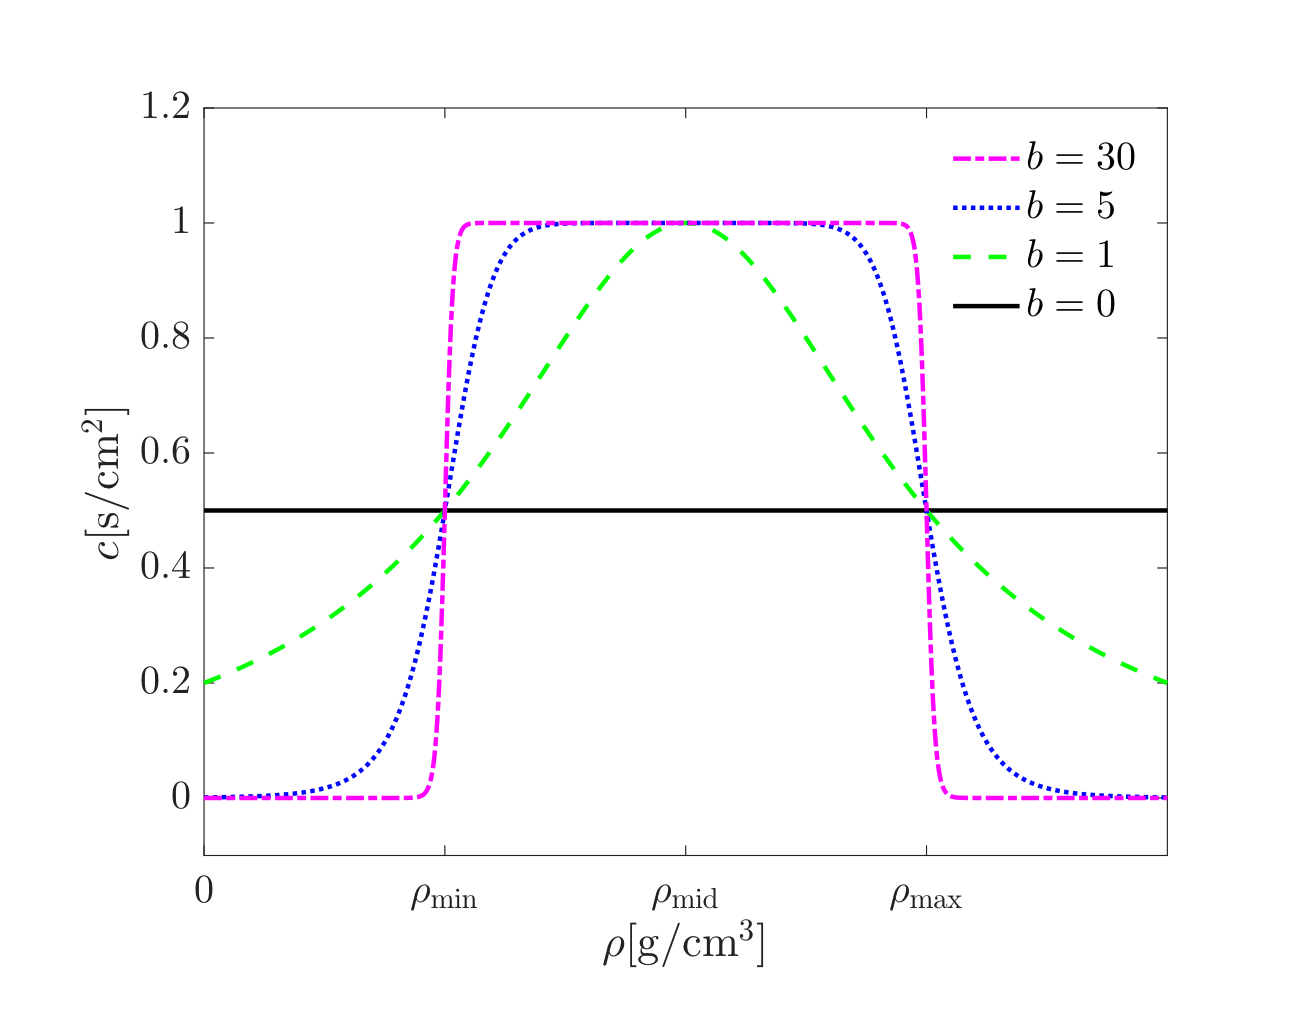
\includegraphics[width=7cm]{Figures/graphs/bell_func.png}
		\caption{Bell function plotted for different values of $\mathrm b$. For $\mathrm b \rightarrow \infty$ the bounds for $ \rho{^\mathrm{min}}$ and $ \rho{^\mathrm{max}}$ sharpen.}
		\label{fig:bell_func}
	\end{centering}
\end{figure}
In the context of porous materials like bones, the free energy $\psi$ is equal to:
\begin{equation}
\psi_{0}=\left[\frac{\rho}{\rho_{0}^{\ast}}\right]^{n}\psi_{0}^{\mathrm{neo}},
\label{eq:free_energ}
\end{equation}
where Helmholtz free energy $\psi$ was chosen to be of Neo-hookean type, which is expressed in terms of the right Cauchy-Green deformation tensor: 
\begin{equation}
\psi_{0}^{\mathrm{neo}}=\frac{\mu}{2}\left[\textrm{tr}(\mathbf{C})-3\right]-\mu\ln(\sqrt{\det\mathbf{C}})+\frac{\lambda}{2}\ln^{2}(\sqrt{\det\mathbf{C}})
\end{equation}
$\mu$ and $\nu$ are the Lam\'e constants. Moreover, the exponent $n$ typically varies between $1 \leq n \leq 3.5$ depending on the porosity of the material \citep{Gibson2005}.
Finally, to iteratively solve the system of nonlinear equations monolithic solution scheme is chosen. Following classical Newton method, both mass and momentum balance equations are linearised. To ensure quadratic convergence of the algorithm, the consistent material tangent matrix is derived by means of automatic differentiation provided with ADOL-C library~\citep{Walther2009}. For the time discretisation of the governing equations, implicit backward Euler method was utilised. The application of the proposed model for equine metacarpal is demonstrated by two numerical examples in Section \ref{sec:numerical_examples}.
\section{Density mapping}
\label{sec:dens_mapping}
Subject-specific finite element (FE) modelling has commonly been used to assess the stresses and fracture risk of bones~\citep{poelert2013patient,Helgason2008b,Yosibash2010}. The two crucial components of subject-specific FE models- model geometry and material properties, can be derived from computed tomography (CT) datasets. Generation of the three-dimensional (3D) geometry of a~bone segment with an accurate material distribution from CT data might be troublesome and time-consuming depending complexity of the considered bone. In this contribution, a new approach to assign bone density from CT scan datasets into FE models is presented. Most of the previously proposed density mapping algorithms simply average~\citep{zannoni1999material} or integrate~\citep{taddei2007material, schileo2008subject} voxel data from CT scans onto finite elements supplying a constant density within their volume. Herein, the data is spatially approximated by using Moving Least Squares (MLS) method. It provides smooth density field and gradient over the entire domain which significantly reduces the noise and improves the quality of FE solution. 
\subsection{Moving least squares}
\label{sec:mwls}
The moving least squares approximation is a method for constructing interpolation functions on a set of nodes and is widely used for various meshless methods \citep{belytschko1996meshless}. In computer graphics, it is useful for reconstructing a surface from a set of points \citep{lancaster1981surfaces} through  downsampling or upsampling. Numerous studies have also attempted utilize the method within the context of Element-Free Galerkin approach as trial and test functions \citep{belytschko1996dynamic,wong2010meshfree, ullah2013finite}. In this study it is used to approximate density and calculate its gradient obtained from clinical CT scan data. \\
In MLS the local approximation of the field variable $u^h({\boldsymbol {\rm x}})$ is expressed as: 
\begin{equation}
u^h({\boldsymbol {\rm x}})=\sum^m_{j=1}p_j({\boldsymbol {\rm x}} )a_j({\boldsymbol {\rm x}} ) =\mathbf p^{\rm T}({\boldsymbol {\rm x}} )\mathbf a({\boldsymbol {\rm x}} )
\label{eq:mwls_approx}
\end{equation}
where $\mathbf p({\boldsymbol {\rm x}})$ is the vector of complete basis functions with order $m$ and $\mathbf a({\boldsymbol {\rm x}})$ is the vector of unknowns and in the case of MLS approximation which is also a function of spatial coordinates, ${\boldsymbol {\rm x}}$, unlike in conventional Least Squares method where $\mathbf a({\boldsymbol {\rm x}})$ is held constant. 
The polynomial basis functions $\mathbf p({\boldsymbol {\rm x}})$ are built form Pascal's pyramid. 
In the current implementation three types of the basis functions are used as follows:
\begin{equation*}
\mathbf p^{\rm T}({\boldsymbol {\rm x}})  = \mathbf p^{\rm T}(x,y,z)= [1], \quad m=1,
\end{equation*}
\begin{equation*}
\mathbf p^{\rm T}({\boldsymbol {\rm x}}) = \mathbf p^{\rm T}(x,y,z)= [1,x,y,z], \quad m=4,
\end{equation*}
\begin{equation}\label{eq:mwls_basis}
\mathbf p^{\rm T}({{\boldsymbol {\rm x}}}) = \mathbf p^{\rm T}(x,y,z)= [1,x,y,z,xy,yz,zx,x^2,y^2,z^2], \quad m=10
\end{equation}
Moving on, the vector of unknowns $\mathbf a({\boldsymbol {\rm x}}) = \Big[ a_1({\boldsymbol {\rm x}} )\quad a_2({\boldsymbol {\rm x}} )\quad\dots \quad a_m({\boldsymbol {\rm x}} ) \Big]$ in Equation (\ref{eq:mwls_approx}) can be obtained from a minimization of weighted discrete $L_2$ norm:
\begin{equation}
J({{\boldsymbol {\rm x}}})=\frac{1}{2} \sum_i^n w_i({{\boldsymbol {\rm x}}}) \left( \mathbf p^{\rm T} ({\boldsymbol {\rm x}}_i)\mathbf a({\boldsymbol {\rm x}}) - u_i \right)^2
\label{eq:mwls_l2}
\end{equation}
where $u_i$,${\boldsymbol {\rm x}}_i $, $w_i({{\boldsymbol {\rm x}}})$ are a nodal parameter, coordinate and a weight function of node $i$, respectively, and $n$ is the number of nodes with $w_i(\mathrm) > 0$; i.e. the nodes belonging to the nodal influence domain of point $x$. Many types of weight functions can be used for MLS approximation. The domain of influence of a node is an essential concept in a meshless method, as it determines the region in which it has influence. The weight function should be non-zero over a small neighbourhood of a node. For illustrative purposes, a 2D domain of influence is presented in Figure \ref{fig:weight_func}.
\begin{figure}[h!]
	\begin{centering}
		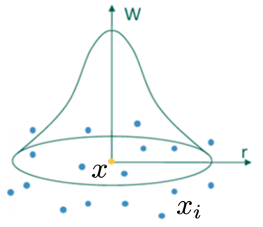
\includegraphics[width=5cm]{Figures/weight_func.png}
		\caption{Example of a weight function and its influence domain. It can be recognized that such function is smooth, non-negative and reaches maximum at the considered node and decrease with the distance $|| {\boldsymbol {\rm x}} - {\boldsymbol {\rm x}}_i||$ from the node. Outside of the influence domain of a node has a constant value of zero. Typically, the size of the domain is determined by searching for enough neighbour nodes such that matrix $\mathbf A$ in Equation (\ref{eq:mwls_system}) is invertible.}
		\label{fig:weight_func}
	\end{centering}
\end{figure}
As one possibility among others, commonly used in the meshless methods  \citep{belytschko1996meshless}, one-dimensional quartic spline was chosen in this work
\begin{equation}
w(||{\boldsymbol {\rm x}}-{\boldsymbol {\rm x}}_i||)=w(r)=\begin{cases} 1-6r^2+8r^3-3r^4 & \mathrm{for} \, r \leq 1\\ 0 & \mathrm{for} \, r > 0 \end{cases}
\end{equation}
and its derivative with respect to the spatial coordinates, which is also required later on.
\begin{equation}
\frac{dw}{d{\boldsymbol {\rm x}}}= \frac{dw}{dr}\frac{dr}{d{\boldsymbol {\rm x}}} =\begin{cases} (-12r +24r^2 -12 r^3) \,  & \mathrm{for} \, r \leq 1, \\ 0 & \mathrm{for} \, r > 0  \end{cases}
\end{equation}
Here $r = ||{\boldsymbol {\rm x}}-{\boldsymbol {\rm x}}_i||/d_{\rm {mi}} $ is the normalised radius, where the distance between the node $i$  and point of interest $x$ is divided by scaling parameter $d_{\rm {mi}}$. This coefficient is governing the size of influence domain at given node. 
The minimisation of norm $J$ in Equation (\ref{eq:mwls_l2}) is found by ${\partial J}/{\partial \mathbf a}$ and leads to a system of linear equations as:
\begin{equation}
\mathbf{ { A }} ({\boldsymbol {\rm x}}) \mathbf{ { a}} ({\boldsymbol {\rm x}}) = \mathbf{ { B }}({\boldsymbol {\rm x}}) \mathbf{ { u}}
\end{equation} \label{eq:mwls_system}
where matrices $\mathbf{ { A }}({\boldsymbol {\rm x}})$ and \textbf{$\mathbf{ { B}}({\boldsymbol {\rm x}})$} are of size $(m \times m )$ and $(m \times n )$ and are defined as follows:
\begin{equation} 
\begin{aligned}
& \mathbf{ { A }}({\boldsymbol {\rm x}}) = \sum_i^n w_i ({\boldsymbol {\rm x}})\mathbf{p} (\mathrm  x_i)\mathbf p^{\rm T} ({\boldsymbol {\rm x}}_i) \\
& \mathbf{ { B }}({\boldsymbol {\rm x}}) = \Big[   w_1({\boldsymbol {\rm x}}) \mathbf p ({\boldsymbol {\rm x}}_1) \quad w_2({\boldsymbol {\rm x}}) \mathbf p ({\boldsymbol {\rm x}}_2) \quad \dots \quad  w_n({\boldsymbol {\rm x}}) \mathbf p ({\boldsymbol {\rm x}}_n)  \Big]
\end{aligned}
\end{equation}
and $\mathbf u$ is $(n \times 1)$ vector of nodal parameters given as 
\begin{equation}
\mathbf u = \big[ u_1 \quad u_2 \quad \dots \quad u_n \big]^{\rm T}
\end{equation}
Next, Eq. (\ref{eq:mwls_approx}) combined with Eq. (\ref{eq:mwls_system}) can be rewritten as 
\begin{equation}
u^h({\boldsymbol {\rm x}} )=\sum^n_{i=1} \phi_i({\boldsymbol {\rm x}}) u_i = \mathbf \phi^{\rm T} ({\boldsymbol {\rm x}}) \mathbf u
\end{equation}
where $ \mathbf \phi ({\boldsymbol {\rm x}})$ is the vector of shape functions.
\begin{equation}
\mathbf \phi ({\boldsymbol {\rm x}}) = \mathbf p^{\rm T} ({\boldsymbol {\rm x}}) \mathbf{A}^{-1} ({\boldsymbol {\rm x}}) \mathbf B ({\boldsymbol {\rm x}}) \mathbf u
\end{equation}
For approximating the field of density, it would be of benefit to calculate its gradient as well. Therefore, the first derivative of the shape function with respect to the spatial coordinates is derived as follows: 
\begin{equation}
\phi_{,i} = \mathbf p^{\rm T}_{,i} \mathbf A^{-1} \mathbf B + \mathbf p^{\rm T} ( \mathbf A_{,i}^{-1} \mathbf B + \mathbf A^{-1} \mathbf B_{,i} )
\end{equation}
where a comma in the subscript denotes the partial derivative and 
\begin{equation}
\mathbf A_{,i}^{-1} = -\mathbf A^{-1} \mathbf A_{,i} \mathbf A^{-1}
\end{equation}
It is worth to mention that MLS shape functions do not satisfy Kronecker delta property: $\phi_i({\boldsymbol {\rm x}}_j \neq \delta_{ij}) $. The values obtained from the MLS approximation are, therefore, not the same as the nodal values, i.e. $u^h({\boldsymbol {\rm x}}_i) \neq u_i $ as presented in Figure \ref{fig:mwls_approxi}.
\begin{figure}[h!]
	\begin{centering}
		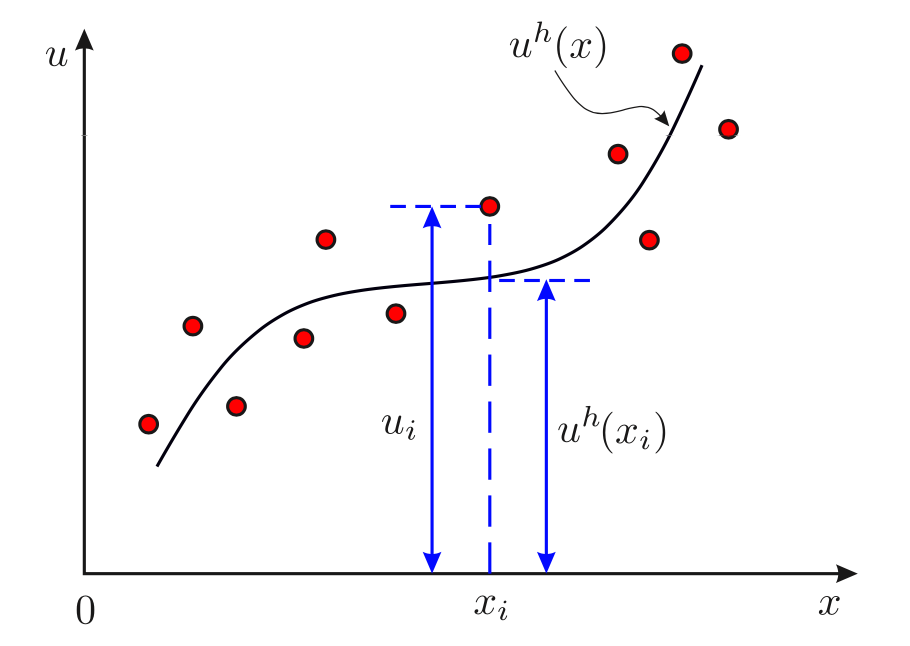
\includegraphics[width=10cm]{Figures/mwls_approxi.png}
		\caption{Moving least squares approximations.}
		\label{fig:mwls_approxi}
	\end{centering}
\end{figure}
%Since the MLS shape functions do not satisfy Kronecker-delta property on the boundaries of the problem; it can be quite a challenge to enforce essential boundary conditions, however, here approximation is used for simple mapping hence this problem can be neglected. 
One of the concerns arising when analysing medical images are Partial Volume Artifacts \citep{adams2009quantitative}. To eliminate mapping spurious bone densities, some researchers proposed to 
redefine data at any node of the mesh surface to data assigned on the nearest internal node \citep{helgason2008modified, chen2010new} or resurface the mesh geometry \citep{peleg2014can}. In this study, a more elegant solution is proposed; every CT scan data point positioned outside the geometry of the bone is simply removed from the domain of influence, thereby only points that fall inside the volume are approximated. 
%Determining whether a given point is inside a polyhedron is a classic computer graphics problem.  It can be solved by casting a ray originating from the given point to an arbitrary direction and determine the number of intersections of the ray with the polyhedron. If the ray intersects the shape an even number of times, then the point is outside the shape. It is important to choose a random direction. (should I describe why based on measure theory?) In MoFEM implementation standard C++ $rand()$ function was used, however without the seed in order to ensure that the code remains deterministic. 
The procedure is computationally expensive, however it has to be performed only once for each influence domain and can be easily parallelized. %is 'embarrasingly parrallel' 
\section{Release energy rate of remodelled bones}
Various theories exist in the literature regarding failure criteria for bone tissue. Commonly researchers attempt to estimate the fracture risk within the framework of finite element analysis. In particular, subject-specific FEM models could potentially quantify how far the bone is from failure under given loading scenario. However, this still remains an open challenge. \\
In recent years, the main focus in bone mechanics was in the use of different strength criteria for failure initialization. The most commonly adopted were based on stress \citep{keyak2005predicting} or strain measures \citep{schileo2008subject} assuming the bone failure under the von Mises, the Drucker-Prager or maximum principal strain and maximum principal stress yield criterion \citep{yosibash2010predicting}. The experimental validations for such simplified models show that they have a significant spread in the predicted failure. The percentage error in the majority of studies report is between 10 and 20\% \citep{van2014accurately}. \\
The variation could be explained due to main attention on the local failure initialization, rather than on the prediction of the propagation. The brittle fracturing process of the bone is far more important and might be crucial for understanding the genesis and complete pattern of the fracture, in particular for fatigue fractures \citep{gupta2008fracture}. Due to many limitations (like usage of 2D geometry \citep{bettamer2017using}, not taking into account bone heterogeneity \citep{gasser2007numerical}), studies in the past have failed to deliver an applicable modelling method to predict the complete fracture pattern of bone. \\
Many methods are currently available to numerically solve the problem of fracture initiation and growth. They can be divided into two categories: discrete and smeared approaches. Discrete crack models originally were limited to describe crack formation only on element boundaries \citep{Scordelis1967}. More recently, in the presence of automatic mesh generators, the extended finite element method (xFEM) separated the crack path from underlying mesh, see e.g. \citep{Belytschko1999} where xFEM was applied to model brittle fracture. Another novel approach in isogeometric analysis field introduces knot insertions that lower the order of continuity to introduce cracks in solids \citep{Hosseini2014}. The continuum damage, or diffused crack approach, incorporates a damage parameter into the model that controls the strength of the material. An advantage of this approach is that it does not require interface tracking since the damage parameter varies continuously over the domain (see, e.g. \citep{deBorst2004}). Closely related to continuum damage models are the phase-field models which have become extremely popular over the last decade. The numerical solution of these models is based on an approximate potential developed by Mumford \citep{Mumford1989}. The main advantage is that the fracture problem can be described purely by partial differential equations \citep{Miehe2010a,Borst2014}. \\
This paper presents a modified formulation and associated computational framework for brittle fracture in elastic solids within the context of configurational mechanics in heterogeneous materials like bones, extending the authors' previous work \citep{kaczmarczyk2017energy}. Configurational mechanics utilises a concept of material (configurational) forces originally introduced by Eshelby~\citep{eshelby1951force}. Unlike physical forces, material forces act on the material manifold and represent the tendency of imperfections like cracks, voids or material inhomogeneities to move relative to the surrounding material. The past two decades have seen a growing interest in this approach for analysis of material imperfections \citep{maugin2016configurational} and in particular for evaluation of crack-driving forces \citep{steinmann2001application, ozencc2016configurational, kaczmarczyk2017energy}. Such implementations in the framework of Finite Element analysis have proven to be accurate, robust and capable of handling a propagation of complex 3D non-planar crack surfaces. However, until recently the approach have never been used to effectively assess material forces in a heterogeneous body with a crack. For this purpose, in the current study, additional material forces arising from inhomogeneities are introduced into the formulation. Such modification allows for identification of the liability of an arbitrary crack to propagate and in the future can be extended to simulate full fracture propagation in bone. An additional goal is to investigate bone failure at different stages of bone adaptation, utilising the results from bone remodelling analysis or data directly taken from CT scans. Similar concept of combined remodelling and fracture analyses has been presented before \citep{hambli2013integrated}. However, it utilised a different remodelling model and continuum damage mechanics approach for fracture, both of which require many more parameters to calibrate. 
\subsection{Kinematics}\label{sec:Kinematics}
In the context of configurational mechanics, an elastic body with an initial crack, as visualised in Figure \ref{fig:frac_kinematics}, is considered. To independently observe the deformation of the material in physical space $\Omega_t$ and the evolution of the crack surface in material space $\mathcal B_t $ it is convenient to decompose the problem into separate configurations. First, propagation of the crack is described by the mapping from the reference configuration to the current material domain, $\Xi$. Next, purely elastic deformation is mapped from the current material to spatial domain, $\mathbf \phi$. Let $\mathbf x = \phi(\mathbf X,t)$ describe the motion of the body, which transforms material positions $\mathbf X$ to their spatial counterparts $\mathbf x$. The physical displacements are derived as follows:
\begin{equation}
\mathbf u = \mathbf x - \mathbf X
\end{equation}
The reference configuration represents the body before crack extensions with mapping $\mathbf \Xi( { \boldsymbol {\rm \chi}}, t)$ of the reference coordinates ${ \boldsymbol {\rm \chi}}$ on to the material coordinates $\mathbf X$. This mapping describes a material structural change like extensions of the crack as a result of the crack front movement. 
\begin{figure}[h!]
	\begin{centering}
		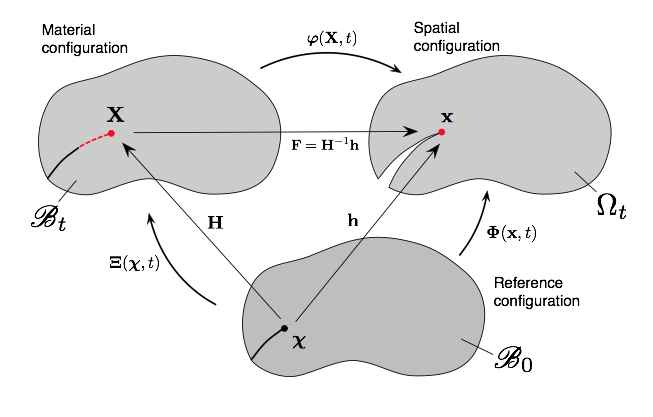
\includegraphics[width=10cm]{Figures/frac_kinematics.png}
		\caption{Decomposition of crack propagation in an elastically deforming body.}
		\label{fig:frac_kinematics}
	\end{centering}
\end{figure}
Finally, mapping $\mathbf \Phi ({ \boldsymbol {\rm \chi}},t)$ transforms reference coordinates on to the spatial coordinates ${\boldsymbol {\rm x}}$. The current material and spatial displacements are:
\begin{equation}
\mathbf W = \mathbf X - { \boldsymbol {\rm \chi}} \quad \mathrm{and} \quad \mathbf w = \mathbf x - { \boldsymbol {\rm \chi}}
\end{equation}
$\mathbf H$ and $\mathbf h$  gradients of the material and spatial maps are defined as:
\begin{equation}
\mathbf H = \nabla_{\boldsymbol {\rm \chi}} {\boldsymbol {\rm \Xi}}, \quad \mathbf  h =   \nabla_{\boldsymbol {\rm \chi}} {\boldsymbol {\rm \Phi}}
\end{equation}
Corresponding deformation gradient $\mathbf F $ is derived as follows:
\begin{equation}
\mathbf F =  { \boldsymbol {\rm \chi}} \phi=\mathbf h \mathbf H^{-1}
\end{equation}
Since physical material cannot penetrate itself or reverse the orientation of material coordinates, the following constraint has to be imposed:
\begin{equation}
{\mathrm {det}} \mathbf {F} = \frac{\mathrm {det} (\mathbf h)}{\mathrm {det} (\mathbf H)} > 0
\end{equation}
Moving on, the velocity of a material point $\mathbf X$ and the time derivative of the deformation gradient have the following form:
\begin{equation}\label{eq:crack_disp}
{\dot {\boldsymbol {\rm u} } } = {\dot {\boldsymbol {\rm w} } } - \mathbf F{\dot {\boldsymbol {\rm W} } }
\end{equation}
and
\begin{equation}\label{eq:crack_def_grad}
{\dot {\boldsymbol {\rm F} } } = \nabla_{\mathbf X} {\dot {\boldsymbol {\rm w} } } - \mathbf F \nabla_{\mathbf X } {\dot {\boldsymbol {\rm W} } }
\end{equation}
\begin{figure}
	\begin{centering}
		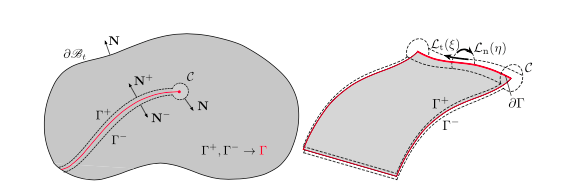
\includegraphics[width=10cm]{Figures/frac_crack_con.png}
		\caption{Crack construction \citep{kaczmarczyk2017energy}.}
		\label{fig:frac_crack_con}
	\end{centering}
\end{figure}
\subsection{Crack front}
The crack surface is denoted as $\Gamma$ with a crack front $\partial \Gamma$, see Figure \ref{fig:frac_crack_con}.  Following \citep{kaczmarczyk2014three}, a kinematic relationship between the change in crack surface area $\dot A_\Gamma$ and the crack front velocity $\mathbf{\dot W}$ can be defined as:
\begin{equation}\label{eq:crack_front}
\dot A_\Gamma = \int_{\partial \Gamma} \mathbf A_{\partial \Gamma} \cdot {\dot {\boldsymbol {\rm W} } } \mathrm d L 
\end{equation}
where $ \mathbf A_{\partial \Gamma}$ is a kinematic state variable that defines the current crack front orientation. It should be noted that any change in the crack surface area $\dot A_\Gamma $ and the crack front velocity $\mathbf {\dot W}$ in the material configuration can only take place when the crack propagates. 
%\begin{equation}
%\mathbf \Xi : \mathcal B_0 \to \mathcal B_t, \quad \mathbf X = \mathbf \Xi(\mathbf \chi, t)
%\end{equation}
\subsection{Dissipation of energy at the crack front}
Crack propagation problem can be considered as a thermodynamic system consisting of a solid deformable body with an imperfection. Traction applied on the boundary of the body $\partial \mathcal B_t$ performs work on the system. Following the first law of thermodynamics, it can be assumed that all energy within the volume of the body is used for mechanical work and it can be expressed as 
\begin{equation}
\int_{\partial \mathcal B_t} {\dot {\boldsymbol {\rm u} } } \cdot \mathbf t \mathrm d S = \gamma \dot A_\Gamma +{\frac{\mathrm d}{\mathrm d t }} \int_{\mathcal B_t} \Psi(\mathbf F) \mathrm d V
\end{equation}
where the left hand side is the power of external work. The first therm on the right hand side is the rate of the crack surface energy and the last term is the rate of internal body energy. $\mathbf t$ is the external traction vector, $\gamma $ is the surface energy $[ {\rm{N m}}^{-1} ]$ and $\Psi$ is the free energy density function. Next, by substituting Equations (\ref{eq:crack_disp}),(\ref{eq:crack_def_grad}) and (\ref{eq:crack_front}) and given that $\mathrm d \dot V = \nabla _{\mathbf X} \cdot \mathbf{\dot W} \mathrm d V$, the above expression can be reformulated as:
\begin{equation}\label{eq:crack_first_law}
\int_{\partial \mathcal B_t} \big( {\dot {\boldsymbol {\rm w} } } \cdot \mathbf t - {\dot {\boldsymbol {\rm W} } } \cdot \mathbf F^{\rm T} \mathbf t \big) \mathrm d S = \int_{\partial \Gamma } \gamma \mathbf A_{\partial \Gamma} \cdot {\dot {\boldsymbol {\rm W} } } \mathrm d L + \int_{\mathcal B_t} \big( \mathbf P\, \colon \nabla_{\mathbf X} {\dot {\boldsymbol {\rm w} } } +\mathbf  \Sigma\, \colon \nabla_{\mathbf X} {\dot {\boldsymbol {\rm W} } } \big) \mathrm d V 
\end{equation}
where
\begin{equation}
\mathbf P = \frac{\partial \Psi (\mathbf F, \rho)}{\partial \mathbf F} \quad \mathrm{and } \quad \mathbf \Sigma = \Psi(\mathbf F) \mathbf  1 - \mathbf F^{\rm T} \mathbf P
\end{equation}
are the first Piola-Kirchhoff stress and Eshelby stress tensors, respectively. The first one is a well-known driving force for elastic deformation in the spatial domain. It is worth noting that in case of the previously presented bone material model, it also depends on density $\rho$. The Eshelby stress is Piola's material counterpart and is the driving force for local configurational changes in the material domain. Local form of the first law in Equation (\ref{eq:crack_first_law})
can be obtained by applying the divergence theorem to the last integral resulting in the following expression:
\begin{equation}\label{eq:crack_local_gauss}
\begin{aligned}
&  \int_{\partial \Gamma } \gamma \mathbf A_{\partial \Gamma} \cdot {\dot {\boldsymbol {\rm W} } } \mathrm d L = \int_{\mathcal B_t} {\dot {\boldsymbol {\rm w} } } \cdot \big( \nabla_{\mathbf x} \cdot \mathbf P  \big) \mathrm d V + \int_{\mathcal B_t} {\dot {\boldsymbol {\rm W} } } \cdot \big( \nabla_{\mathbf x} \cdot \mathbf \Sigma \big) \mathrm d V \\
& +\int_{\partial \mathcal B_t \cup \Gamma^+ \cup \Gamma^-} {\dot {\boldsymbol {\rm w} } }\cdot \big( \mathbf t - \mathbf{PN}\big) \mathrm  d S + \int_{\partial \mathcal B_t \cup \Gamma^+ \cup \Gamma^-}  {\dot {\boldsymbol {\rm W} } } \cdot \big( \mathbf F^{\rm T} + \mathbf{\Sigma N} \big) \mathrm d S \\
& - \lim_{\mathcal C \to 0} \int_{\mathcal C} {\dot {\boldsymbol {\rm w} } } \cdot \mathbf {PN} \mathrm d S + \lim_{\mathcal C \to 0} \int_{\mathcal C} {\dot {\boldsymbol {\rm W} } } \cdot \mathbf{\Sigma N} \mathrm d S
\end{aligned}
\end{equation}
Moreover, it can be recognised that, in the limit, the surface $\mathcal C$ (Figure \ref{fig:frac_crack_con}) collapses to the crack front $\partial \Gamma $ and integrals over the crack front are simplified as follows:
\begin{equation}
\lim_{\mathcal C \to 0} \int_{\mathcal C} (\cdot ) \mathrm d S = \lim_{\mathcal C \to 0} \int_{\mathcal L_t} \int_{\mathcal L_n} (\cdot) \mathrm d S = \int_{\partial \Gamma} \lim_{|\mathcal{ L }|\to 0} \int_{\mathcal L_n } (\cdot ) \mathrm d S
\end{equation}
The spatial conservation law of linear momentum balance, for any point inside the body, is expressed as follows:
\begin{equation}
\nabla_{\mathbf X} \cdot \mathbf P = 0
\end{equation}
Therefore, the first term on the right-hand side in Equation (\ref{eq:crack_local_gauss}) vanishes. 
However, the material conservation law is not equal to zero in case of heterogeneous materials like bones. Following \citep{kienzler2014configurational}, material defects and inhomogeneities can create additional configurational forces; hence, material momentum balance can be expressed as:
\begin{equation}
\nabla_{\mathbf X } \cdot \mathbf \Sigma = \mathbf f^{\mathrm {inh}}
\end{equation}
where $ \mathbf f^{\mathrm {inh}}$ is a fictitious force, directed from the $ \textit {harder}$ part of the material to the $ \textit {softer}$ part. It represents a vector of the spatial variation of material properties, and in the context of heterogeneous bodies considered in this study it has the following form:
\begin{equation}
\mathbf f^{\mathrm {inh}} = - \left( \frac{\partial \Psi }{ \partial \mathbf X} \right)_{\mathrm{expl}} = - \left. \left( \frac{\partial \Psi}{\partial \rho} \right) \left( \frac{\partial \rho}{\partial \mathbf X} \right) \right|_{\mathbf x= \mathrm{const}}
\end{equation}
where $\Psi$ is the free energy that depends on density as noted in Equation (\ref{eq:free_energ}). Above expression is an explicit derivative - it does not depend on the spatial configuration $\mathbf x$. \\
Furthermore, considering only admissible velocity fields and stress fields in equilibrium with external forces, the following expression can be obtained. 
\begin{equation}
\int_{\partial \Gamma } \gamma \mathbf A_{\partial \Gamma} \cdot {\dot {\boldsymbol {\rm W} } } \mathrm d L -\int_{\partial \Gamma} {\dot {\boldsymbol {\rm W} } } \cdot \lim_{|\mathcal L_n| \to 0 }  \int_{\mathcal L_n } \mathbf{\Sigma N} \mathrm d S  = 0
\end{equation}
The configurational (material) force at the crack front, which is the material counterpart of the spatial internal force vector is defined as:
\begin{equation}
\mathbf G = \lim_{|\mathcal{ L }|\to 0} \int_{\mathcal L_n} \mathbf{ \Sigma N}\, \mathrm d L 
\label{eq:crack_configuration_force}
\end{equation}
It should be noted that for a continuous and homogeneous elastic body, the material force $\mathbf G$ away from the crack should be zero.
Next, the local form of the first law presented in Equation (\ref{eq:crack_local_gauss}) is: 
\begin{equation}\label{eq:crack_local_first_law}
{\dot {\boldsymbol {\rm W} } } \cdot \left( \gamma \mathbf A_{\partial \Gamma} - \mathbf G \right) = 0
\end{equation}
This equation represents the equilibrium condition for the crack front. The term $ \gamma \mathbf A_{ \partial \Gamma }$ can be considered as material resistance. However, the crack evolution is not within the scope of this study. \\
\subsection{Spatial and material discretisation}
The finite element approximation is applied to both the material and physical space:
\begin{equation}
\begin{aligned}
& \mathbf{ X^h} = \mathbf \Phi({\boldsymbol {\rm {\chi}}}) \tilde {\mathbf{ X}}, \quad \mathbf{x^h} = \mathbf{\Phi}({\boldsymbol {\chi}}) {\tilde{\mathbf{x}}} \\
& \mathbf{ W^h} = \mathbf \Phi(\chi) {\dot { \tilde {\boldsymbol {\rm W} } }}, \quad \mathbf{w^h} = \mathbf{\Phi}({\boldsymbol {\chi}}){\dot { \tilde {\boldsymbol {\rm w} } }}
\end{aligned}
\end{equation}
where superscript h indicates approximation and $(\tilde \cdot)$ nodal values. Three-dimensional domains are discretised with tetrahedral finite elements with hierarchical basis functions of arbitrary polynomial order, following the work of Ainsworth and Coyle \citep{Ainsworth2003}. The higher-order approximations are only applied for displacements in the spatial configuration, whereas a linear approximation is used for displacements in the material space. The material and spatial gradients of deformation are expressed as:
\begin{equation}
\mathbf H^h = \mathbf{B_x}(\chi) {\tilde{\mathbf{X}}}, \quad \mathbf h^h = \mathbf{B_x} ({\boldsymbol {\chi}}) { \tilde{\mathbf{x}}}, \quad \mathbf F^h = \mathbf h^h (\mathbf H^h)^{-1} = \mathbf{B_x} \mathbf{\tilde x}
\end{equation}
The residual force vector in spatial domain has the classical form:
\begin{equation}
\mathbf r_s^h = \mathbf f_\mathrm{{ext,s}}^h - \mathbf f_\mathrm{{int,s}}^h
\end{equation}
where $\mathbf f_\mathrm{{ext,s}}^h $ and $  \mathbf f_\mathrm{{int,s}}^h$ are the vectors of internal and external forces, respectively, and take the following format:
\begin{equation}
\mathbf f_\mathrm{{ext,s}}^h = \aoperator_{\text{TRI}}^{n_{\rm {el}}} \int_\text{TRI} \mathbf \Phi^{\rm T} \mathbf t^h \mathrm d S, \quad \mathbf f_\mathrm{{int,s}}^h = \aoperator_{\text{TET}}^{n_{\rm {el}}} \int_\text{TET}  (\mathbf{ B_x})^{\rm T} \mathbf{P}^h \mathrm d V
\end{equation}
Therein, the operator $ \aoperator$ symbolises the assembly of all contributions for tetrahedral and triangular elements. The discretised version of Equation (\ref{eq:crack_configuration_force}) renders the residual force vector in the material domain, expressed as:
\begin{equation}
\mathbf r_m^h = \mathbf f^h_{\text{res}} - \mathbf{\tilde G}^h
\end{equation}
The nodal material forces $\mathbf{\tilde G}^h$ are the driving force for the crack front propagation and have the following form:
\begin{equation}\label{eq:crack_material_force_dis}
\mathbf{\tilde G}^h = \aoperator_{\text{TET}}^{n_{\rm {el}}} \int_\text{TET} (\mathbf{B_x})^{\rm T} \mathbf \Sigma^h +   \left.\left( \frac{\partial \Psi}{\partial \rho} \right)\right|_{\mathbf{x}= \text {const}} \mathbf B^{\rm T} \rho \mathrm \,d V
\end{equation}
The explicit derivative of energy with respect to density in Equation (\ref{eq:crack_material_force_dis}) is derived automatically by means of ADOL-C library~\citep{Walther2009}. Furthermore, $\mathbf f^h_{\text {res}}$ is the vector of nodal material resistance (Griffith) forces, given as:
\begin{equation}
\mathbf f^h_{\text{res}} = \frac{1}{2} (\mathbf{\tilde A}^h_\Gamma)^{\rm T} \mathbf g_c
\end{equation}
where $ \mathbf g_c$ is a vector with zero for all components except those associated with nodes on the crack front, where the value is equal to $g_c$. It is a material parameter specifying the critical threshold of energy release per unit area of the crack surface $\Gamma$, also known as the Griffith energy.
\subsection{Linearised system of equations}
The nonlinear coupled system of equations is linearised and solved monolithically, following a standard Newton-Raphson iterative strategy. \\

\textcolor{red}{The details of this section has to be discussed with Lukasz}

\section{Numerical examples}
\label{sec:numerical_examples}
A numerical example of a full framework for evaluating release energy rate in remodelled bones is presented in this section. First analysis considers the bone adaptation of an equine 3rd metacarpal bone. In the second one, results of mapping data onto FE mesh are presented. The last subsection demonstrates the results of release energy rate for simple finite plate problem and metacarpal bone verifying the implementation. Additionally, convergence study is conducted with and without quarter point elements at the crack tip.
\subsection{Bone adaptation examples}
\label{sec:numerical_examples:bone_adap}
This section covers the example of equine 3rd metacarpal bone adaptation. The full-scale model of equine MCIII bone is derived from CT scan data. The segmented geometry is discretised into 17041 tetrahedral elements. The material parameters used for the following examples are summarised in Table \ref{tab:parameters_mc3}. The values are adopted based on previous studies of human tibia \citep{Pang2012,Waffenschmidt2012}. Higher stiffness of equine bones, derived from mechanical testing studies \citep{Les1994}, is also taken into account. The initial density is homogeneous, since in the thermodynamic-based model, the starting density does not have a significant effect on the final bone density distribution (at biological equilibrium), similar to some other models \citep{kuhl2003theory}. % is not sensitive to the initial density
Boundary conditions are simplified to two representative forces (5 kN each) spanning over a small area based on pressure film studies \citep{Brama2001} as demonstrated in Figure \ref{fig:mc3_BC}. They are often considered as an equivalent of peak force at the mid-stance of a horse gait. %Obviously, with such simplified loading case the analysis is not sufficient to produce any quantitative results regarding remodelling of the metacarpal but rather to demonstrate the potential of this approach. 
Adaptive time stepping provided with PETSc package \citep{petsc-web} is used in all the simulations with starting time step $\Delta t = 0.5$ and maximum and minimum $\Delta t_{\text {max}} = 50$ and $\Delta t_{\text {min}} = 0.05$, respectively.
\begin{table}[h]
	\centering
	\begin{tabular}{lll}
		\hline
		Parameter             & Description                  & Value  \\ \hline
		$E  $                 & Young's modulus              & $4700 \,\mathrm{ [MPa]}$  \citep{Les1994} \\
		$\nu  $               & Poisson ratio                & $0.3 \,\mathrm{ [-]}$ \\
		$\rho_0 ^\ast  $      & Initial density              & $1.0 \,\mathrm{[ g/cm^{3}]}$  \\
		$\psi_{0}^\ast $      & Target energy                & $0.0275\,\mathrm{ [MPa]}$   \citep{Waffenschmidt2012}  \\
		$c$                   & Density growth velocity      & $1.0 \,\mathrm{ [d/cm^{2}]}$   \\
		$m$                   & Algorithmic exponent         & $ 3.25 \,\mathrm{ [-]}$          \\
		$n$                   & Porosity exponent            & $2.25 \,\mathrm{ [-]}$      \citep{Les1994}   \\ 
		\hline
	\end{tabular} 
	\caption{Material parameters used for the simulations of MC3 bone remodelling.}
	\label{tab:parameters_mc3}
\end{table}
\begin{figure}[h!]
	\begin{centering}
		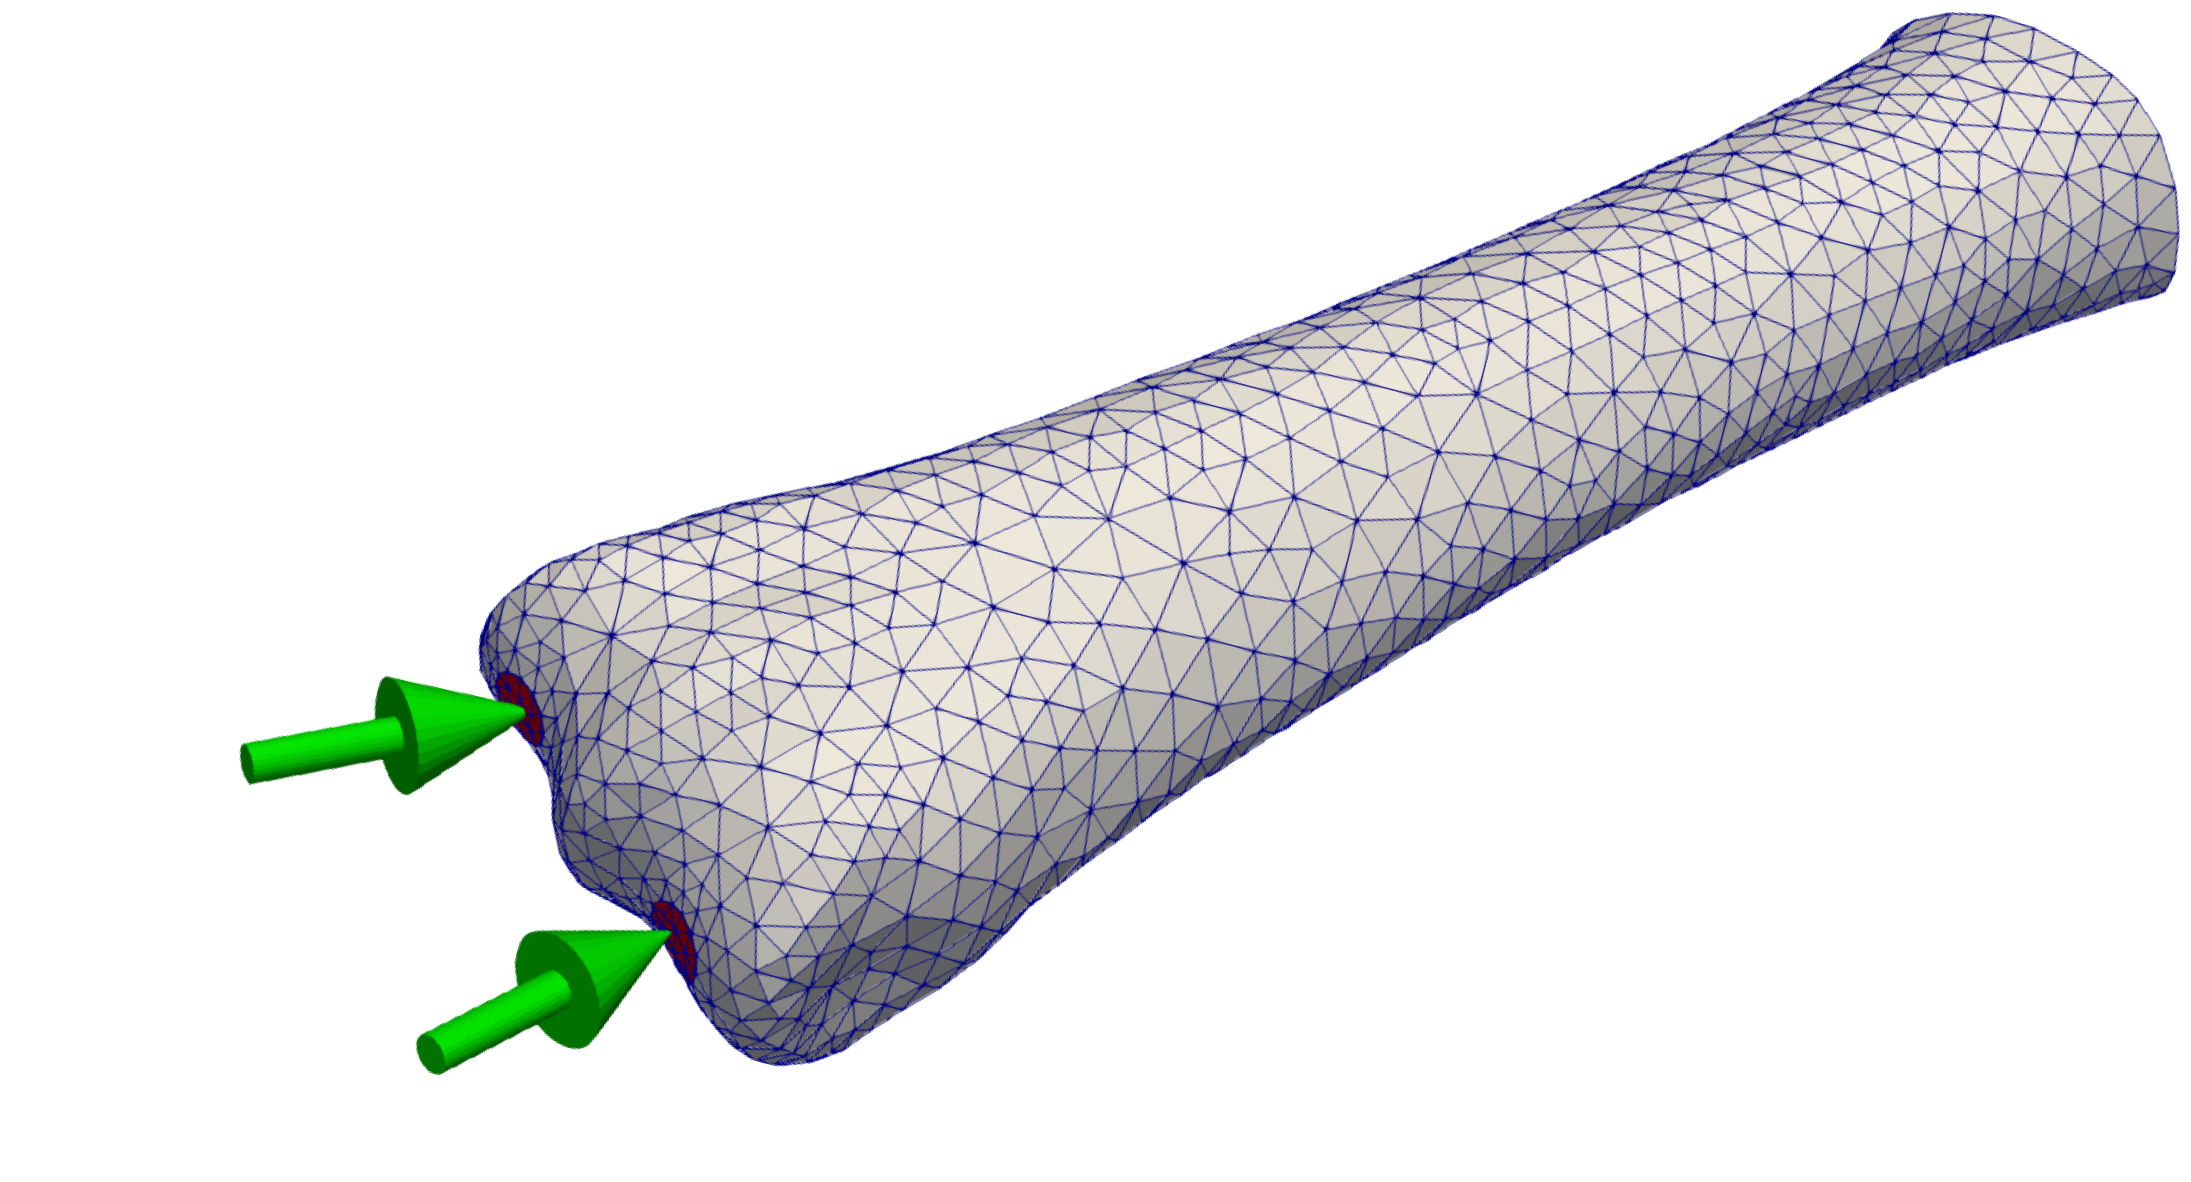
\includegraphics[width=8cm]{Figures/mc3_BC.png}
		\caption{Finite element mesh of the equine 3rd metacarpal bone. The subject specific three-dimensional mesh consists of 14,041 quadratic tetrahedral elements and 70,901 degrees of freedom. To simulate the peak load of a gallop, 5 kN forces are applied on the lateral and medial side of the distal condyle.}
		\label{fig:mc3_BC}
	\end{centering}
\end{figure}
Results of the analysis are presented in Figure \ref{fig:mc3_density} where density maps at five different points in time (0, 10, 40, 100, 700) are visualised. Great densification occurred right after reaching the maximum level of the loading, particularly in the proximity of applied forces, where the high levels of strain energy are expected. In the areas not affected by the loading, material degradation can be observed. After time 100 density levels on entire bone became saturated, biological equilibrium was achieved; hence, no changes in mass appear thereafter. The resulting maximum density has the value of $2.8 \text g \text / {cm}^3$, whereas the minimum is close to zero (unloaded regions).
\begin{figure}[h!]
	\begin{centering}
		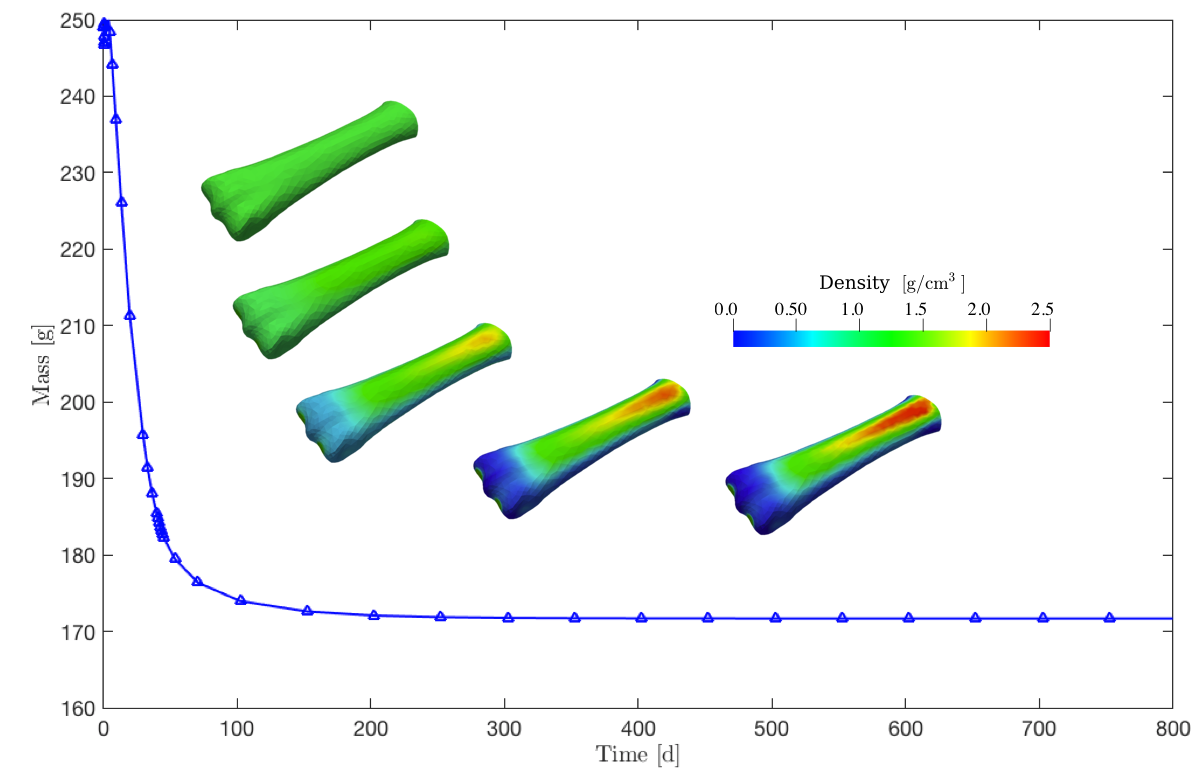
\includegraphics[width=15cm]{Figures/graphs/mc3_density.png}
		\caption{Change in overall mass of the bone over time with density evolution contours in the 3rd metacarpal at five different time points.}
		\label{fig:mc3_density}
	\end{centering}
\end{figure}
When adaptation converges to an equilibrium state, an interesting phenomenon is observed; as a direct consequence of the constitutive Equation \ref{eq:mass_source}, for each density level there is a corresponding value of constant strain energy density $\psi$. This feature can be visualized by plotting the strain energy density on the contours of constant density levels as presented in Figure~\ref{fig:mc3_biol_eq}. 
\begin{figure}[h!]
	\begin{centering}
		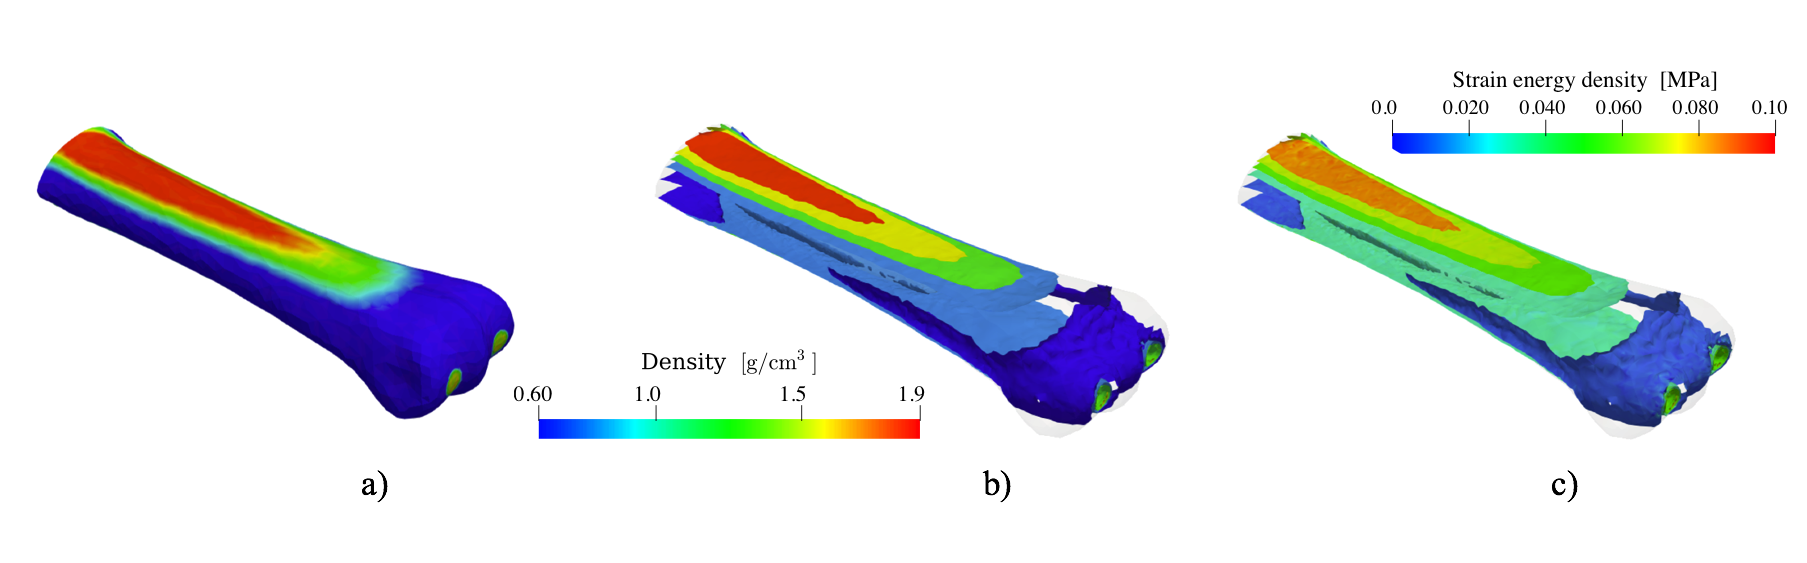
\includegraphics[width=12cm]{Figures/mc3_biol_eq.png}
		\caption{Biological equilibrium state. a) Density map. b) Contours of density. c) Strain energy plotted on contours.}
		\label{fig:mc3_biol_eq}
	\end{centering}
\end{figure}

\subsubsection{Bell function}
\label{sec:bell}
The resulting maximum densities in the analysis demonstrated above are noticeably higher than in the actual equine bones \citep{yamada2015experimental}, whereas minimum density is unrealistically close to zero. There is clearly a need to somewhat constrain upper and lower bounds for density in order to produce more realistic outcomes.
Therefore, in the following section, the results of two analyses with the application of the bell function (see Eq. \ref{eq:bell_function}) are presented. In the first one, the parameters for the function are: $b = 1000$, $\rho_\mathrm{max} = 2.5$, $\rho_\mathrm{min} = 0.3$. All the rest of parameters remain unchanged. The results of the modification are plotted in Figure \ref{fig:density_bell1} below.
\begin{figure}[h!]
	\begin{centering}
		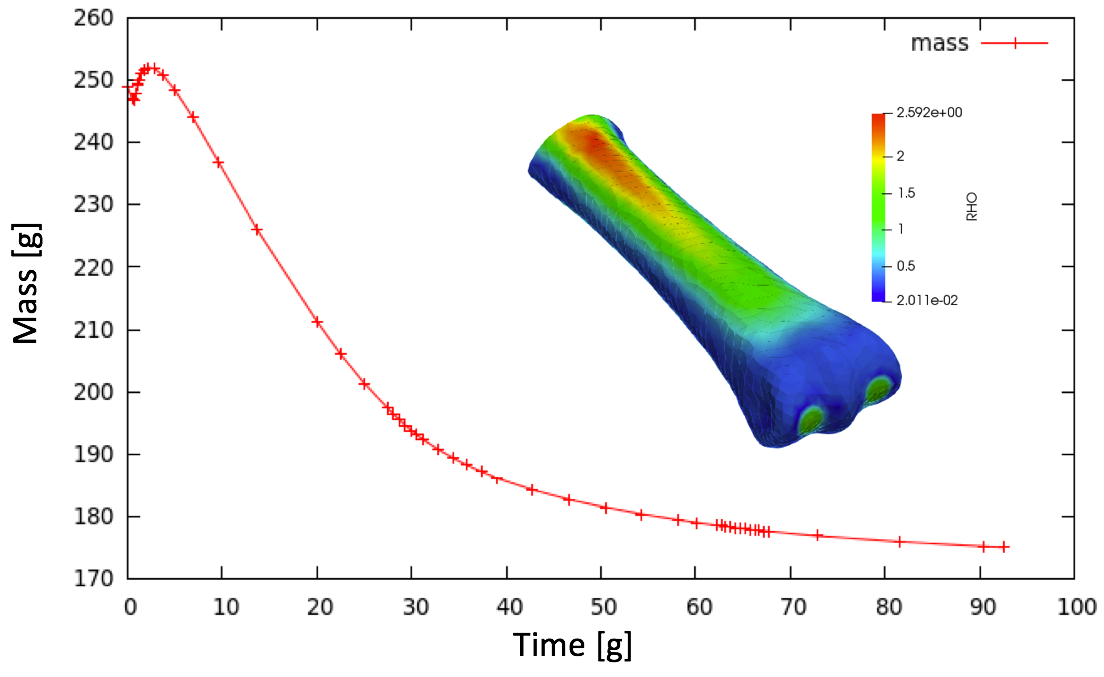
\includegraphics[width=15cm]{Figures/graphs/density_bell1.png}
		\caption{Change in overall mass of the bone over time with applied bell function ($b = 1000$, $\rho_\mathrm{max} = 2.5$, $\rho_\mathrm{min} = 0.3$). Density distribution contours in 3rd metacarpal bone at the last converged step.}
		\label{fig:density_bell1}
	\end{centering}
\end{figure}
The last converged step takes places at $t=93$. By setting a high value of $b$, the transition between densities is very sharp; therefore the algorithm encounters difficulties to obtain derivative of the balance of mass (see Eq. (\ref{eq:mass_balance})), even with adaptive time-stepping. The biological equilibrium cannot be achieved in this case. However, by looking at the range of obtained densities, it is evident that they slowly converge to the same solution as without the restriction of the bell function (Fig. \ref{fig:mc3_density}). 
In the next example, moderate value for the exponent $b$ in the bell function was chosen along with a more strict range for density.
\begin{figure}[h!]
	\begin{centering}
		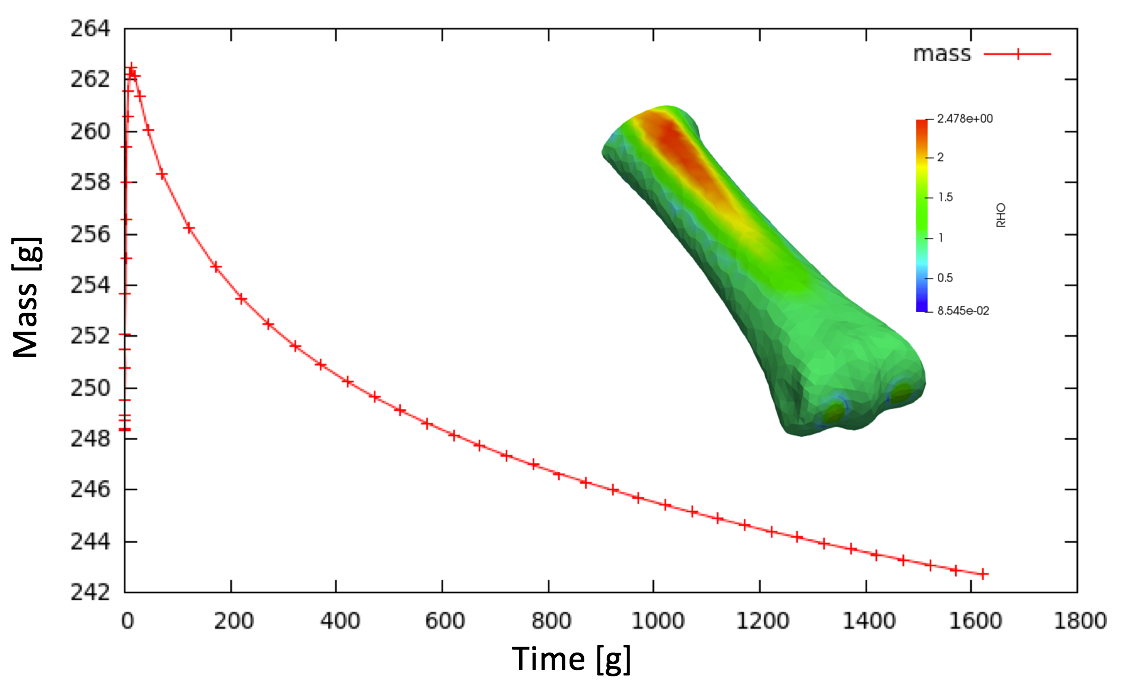
\includegraphics[width=15cm]{Figures/graphs/density_bell2.png}
		\caption{Change in overall mass of the bone over time with applied bell function ($b = 30$, $\rho_\mathrm{max} = 1.8$, $\rho_\mathrm{min} = 1.0$). Density distribution contours in 3rd metacarpal bone at time step $t=1600$.}
		\label{fig:density_bell2}
	\end{centering}
\end{figure}
The plot above demonstrates how set values for bell function influence the results of the analysis. It is evident that with much lower value for exponent $b$, algorithm no longer has problems with calculating the derivative. More strict values of minimum and maximum density clearly have a significant impact on the results. The dense cortical shaft on the dorsal side of the bone is less dense and covers a much larger region. Furthermore, unrealistically low values of densities have been eliminated as well. However, just like the previous case, a tendency can be noticed that the overall solution still converges to the exact same mass (and density distribution) as in the case without the bell function; though it would require significantly more time steps. \\
%In the next sections, the methods will be presented on how to map the resulting density patterns from bone adaptation analysis on different meshes by using moving least squares approximation. Subsequently, the new model will be used to estimate the propensity to fracture, by calculating material forces on the introduced crack tip.
\subsection{MLS mapping examples}
\subsubsection{Simple prism}
In this section, an example of simple mapping of analytical field ($f({\boldsymbol {\rm x}})=x + y^2 + z^3 $) %(simulating CT scan data). 
onto nodes of finite element mesh is presented. At each node of the mesh, the spherical domains of influence are defined (reduced in size for clarity) as shown in Figure \ref{fig:mwlsprism}a). The size of the domain is determined by increasing its radius until matrix $\mathbf A$ in Equation (\ref{eq:mwls_system}) is invertible for all the points. The approximated field data, with its gradient, is saved on corresponding nodes as demonstrated in Figure \ref{fig:mwlsprism}c) for $m=10$. Subsequently, the relative approximation error for gradient is calculated for three cases: constant ($m=1$), linear ($m=4$) and quadratic ($m=10$) basis functions. It is clear from presented results in Figure \ref{fig:prism_error} that constant functions are not sufficient for evaluating the gradient. The maximum error for a linear and quadratic basis has the value of $1.0e-2$ and $1.0e-4$, respectively. These results are satisfactory for the application of mapping data fields onto the mesh and prove the correctness of the implementation.
\begin{figure}[h!]
	\centering
	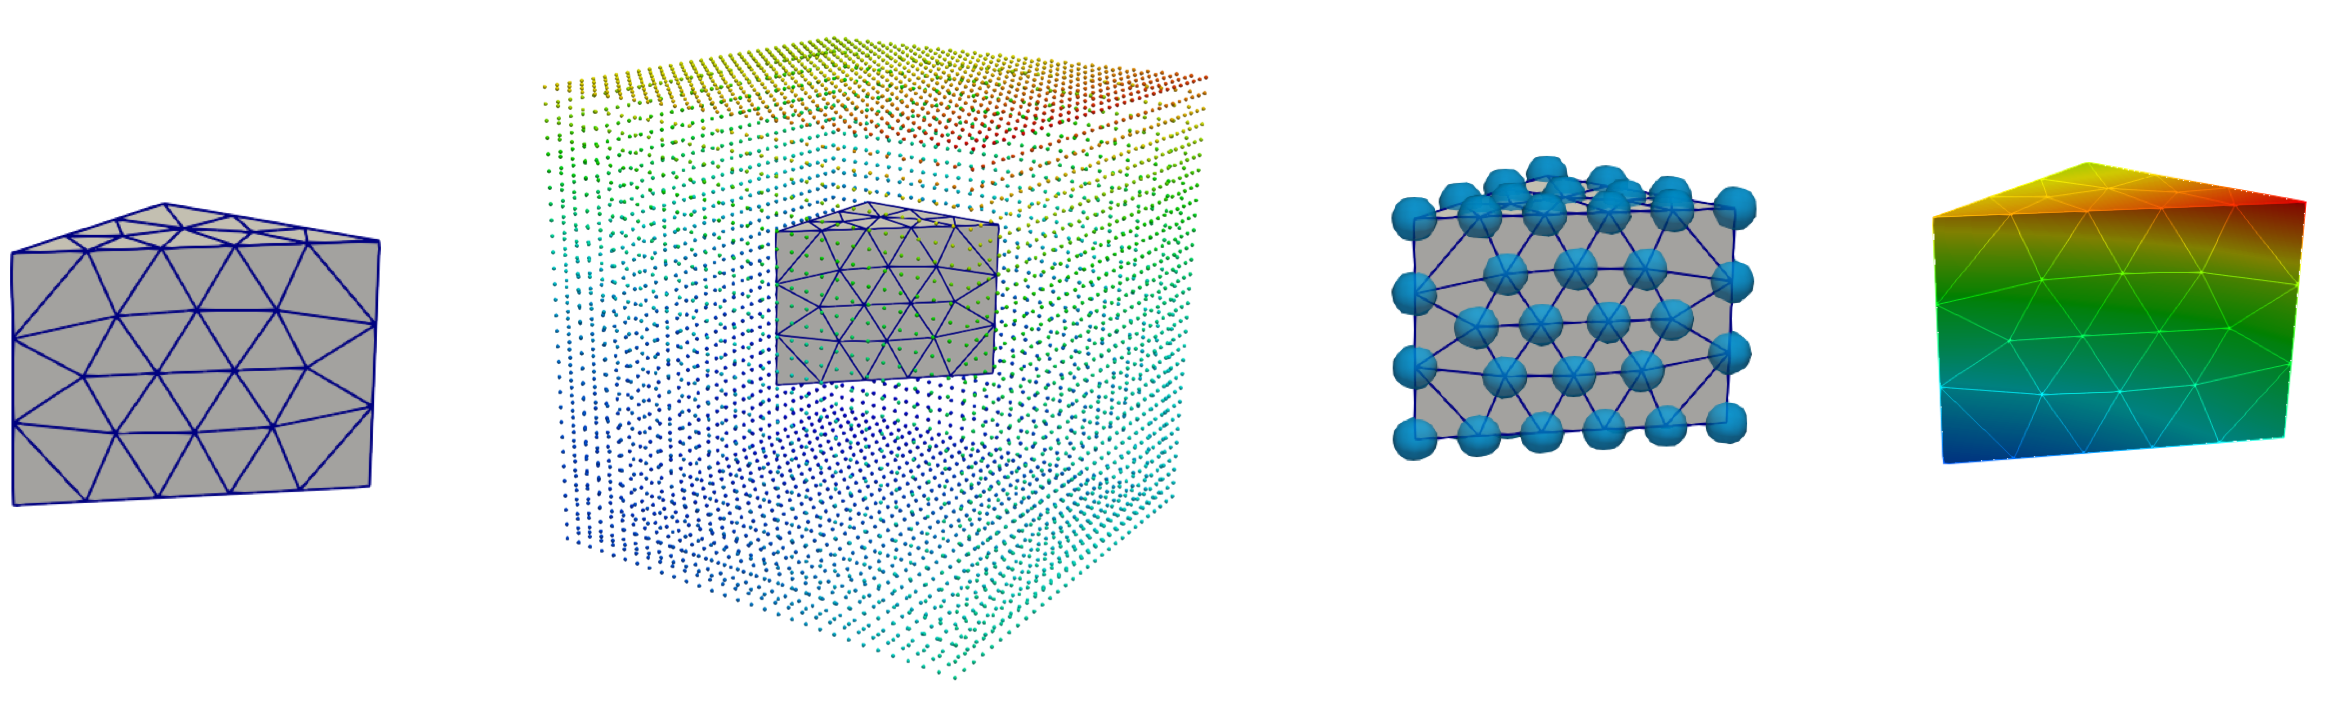
\includegraphics[width=0.8\linewidth]{Figures/mwls_prism.png}
	\caption{a) Finite element tetrahedral mesh with corresponding nodes and spherical domain of influence. b) Analytical field $f({\boldsymbol {\rm x}}) = x + y^2 + z^3$. c) Outcomes of the approximation for $m=10$.}
	\label{fig:mwlsprism}
\end{figure}
\begin{figure}[h!]
	\centering
	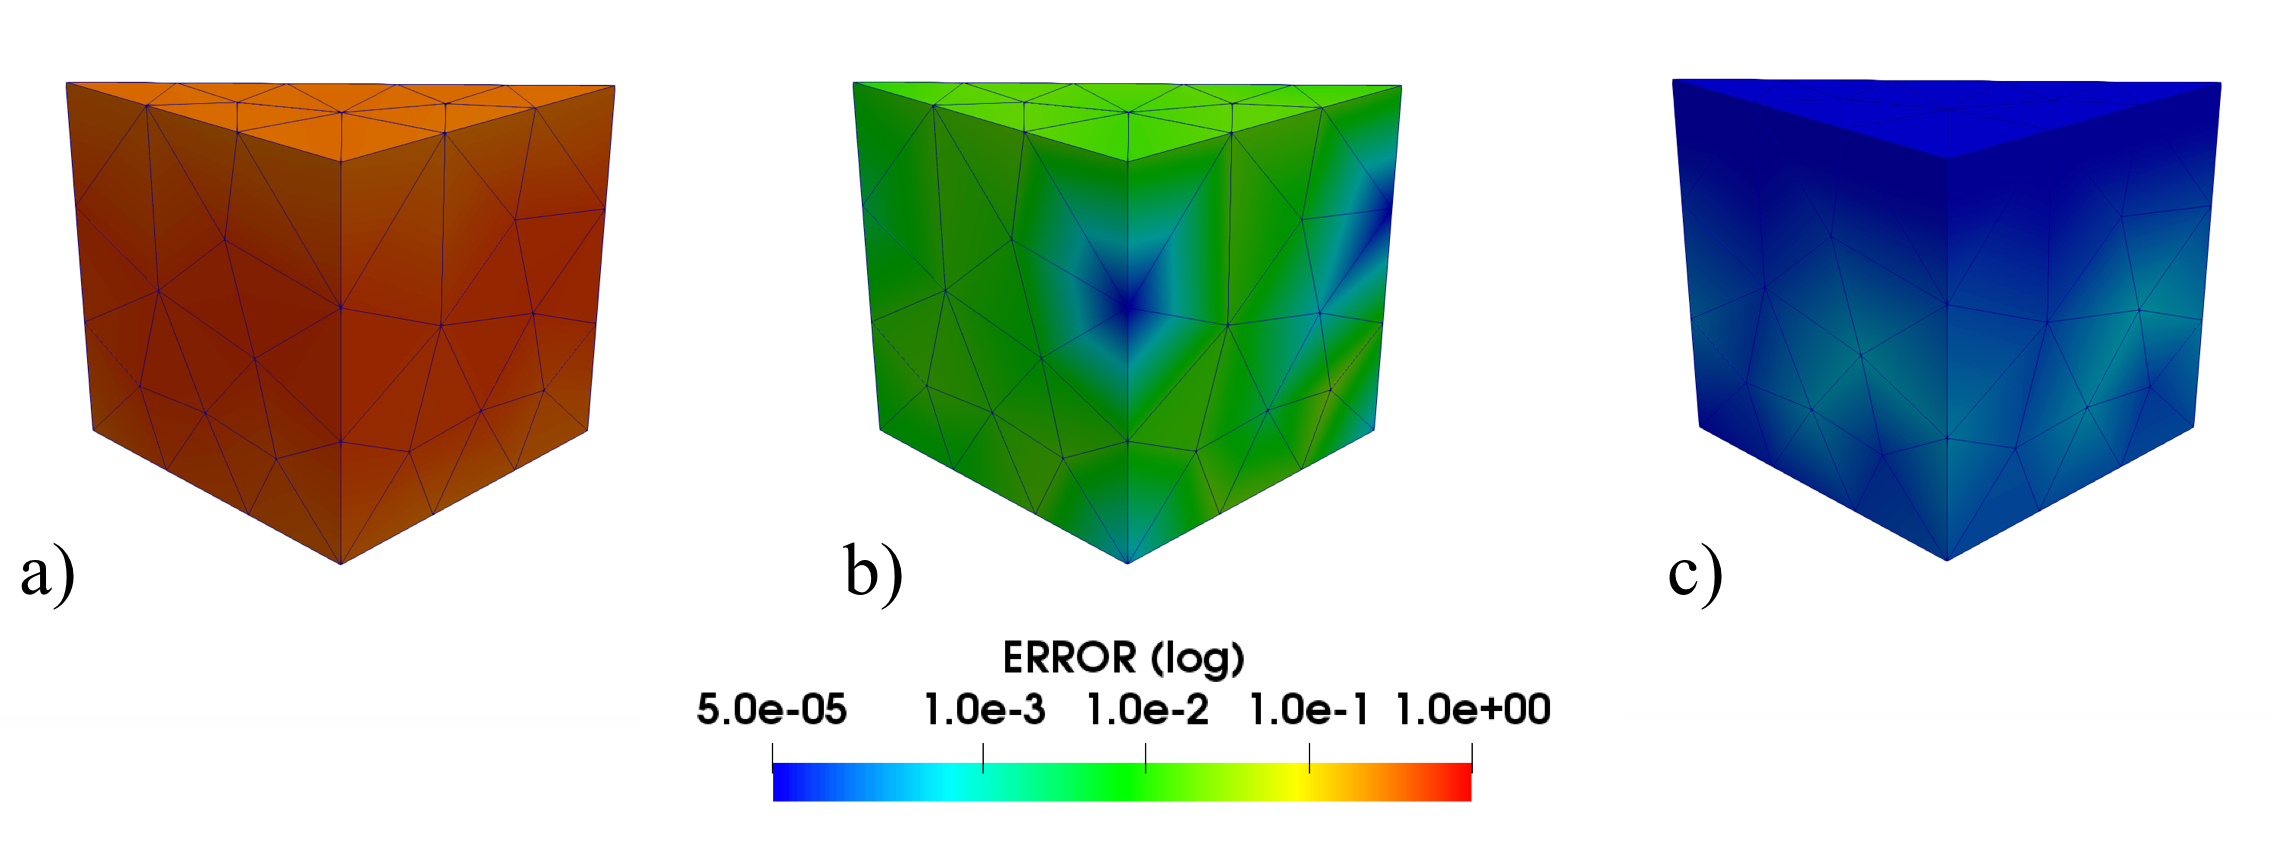
\includegraphics[width=0.8\linewidth]{Figures/prism_error.png}
	\caption{Contour plot of relative error of approximated gradient field for constant a), linear b) and quadratic c) basis functions. The logarithmic scale represents the magnitude of relative error.}
	\label{fig:prism_error}
\end{figure}
\subsubsection{Metacarpal bone}
In this section, the results of density approximation from CT data are presented. Geometry and finite element mesh of an equine 3rd metacarpal bone was obtained in ScanIP (Synopsys Simpleware, Exeter) from medical 3D images. The data was subsequently used to approximate the density values onto finite element mesh nodes by using implemented moving least squares method. The mesh consisted of approximately 7000 tetrahedral elements. \\
\begin{figure}
	\centering
	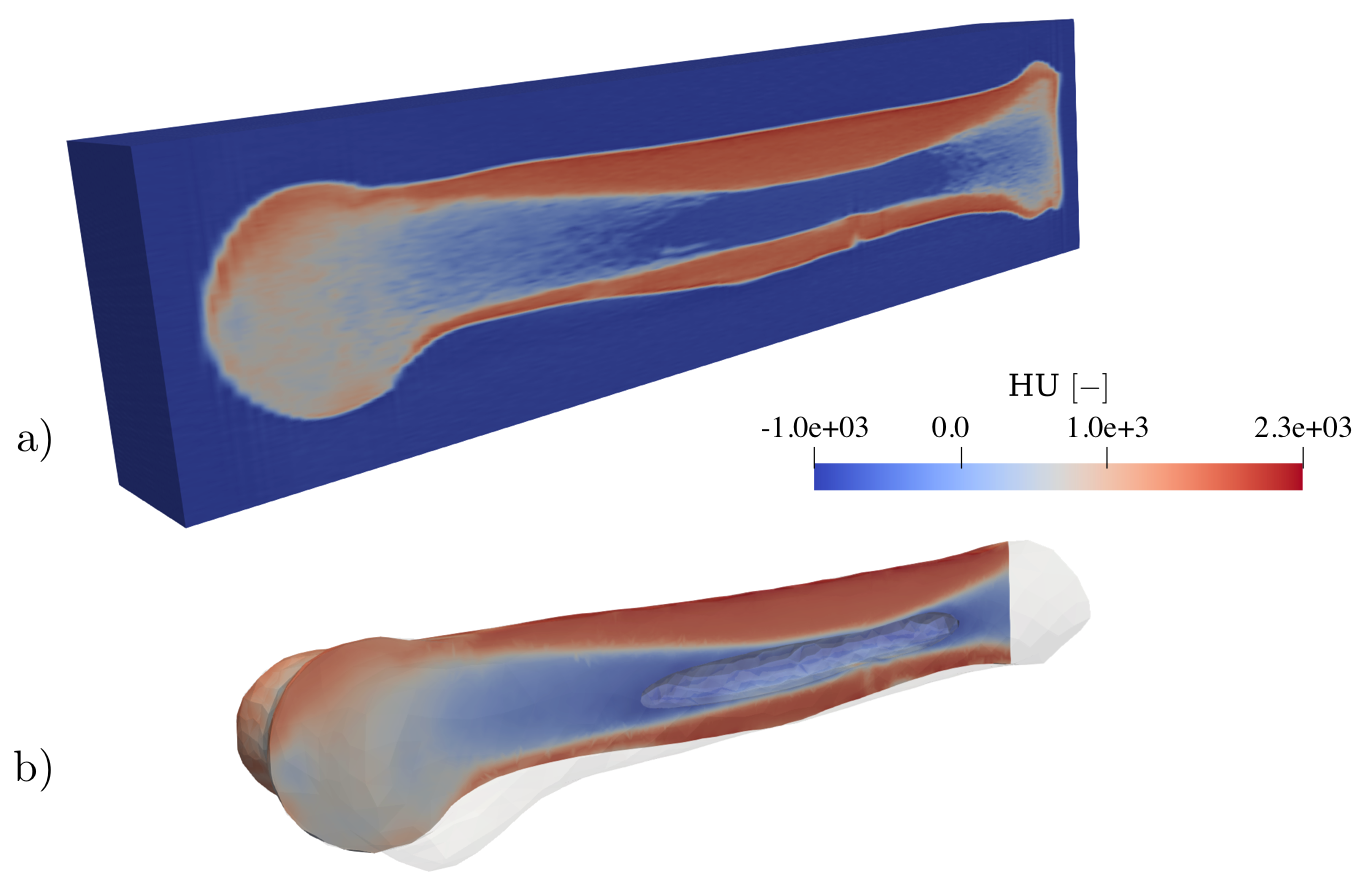
\includegraphics[width=0.5\linewidth]{Figures/mwlsmapping_cross.png}
	\caption{Comparison of a CT data with the corresponding approximation. A cut-view along the Y axis for CT scan data a) and density mapped onto FE mesh. b)}
	\label{fig:mwlsmapping_cross}
\end{figure}
The results of the mapping procedures are presented in Figure \ref{fig:mwlsmapping_cross}. Comparison to CT data and the standard Least Squares (LS) Approximation technique in classical finite element method framework are demonstrated in Figure \ref{fig:mwlsmappingcomparisons}.
\begin{figure}
	\centering
	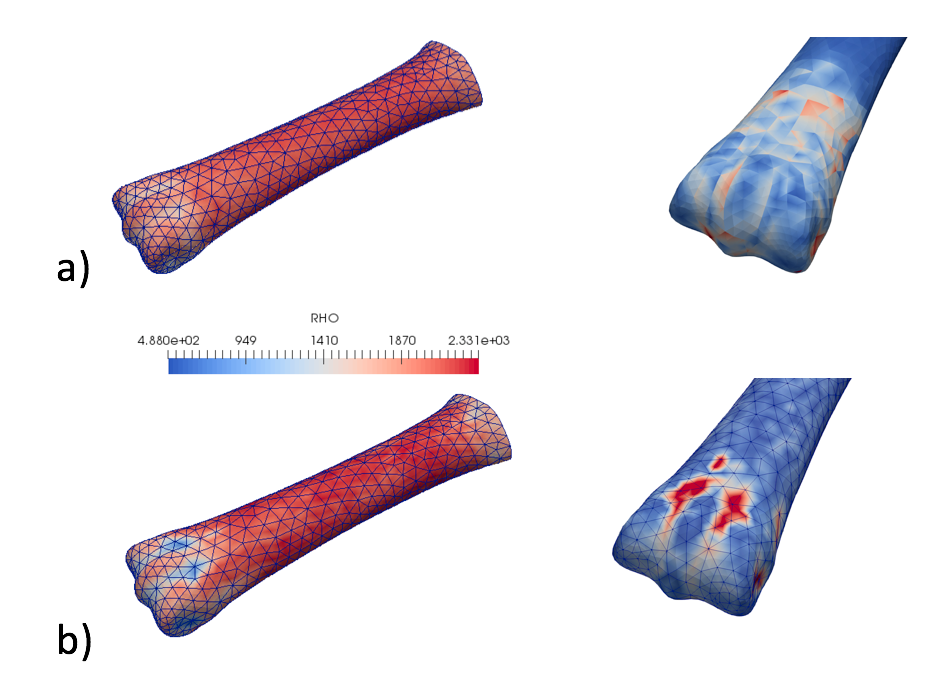
\includegraphics[width=0.7\linewidth]{Figures/mwls_mapping_comparisons.png}
	\caption{Mapping results of bone density (left) and density gradient (right). a) Least squares approximation. b)~Moving least squares approximation.}
	\label{fig:mwlsmappingcomparisons}
\end{figure}
It is clear that mapped density pattern from both methods is very similar. Thanks to the approximation, the obtained field is continuous despite the fact that the mesh is relatively coarse. It is especially beneficial in case of hierarchical basis framework where larger elements with high order approximation are more desired. Classic finite element method provides only $\mathit{C^0}$-continuity; therefore the results of gradients obtained with LS are only piecewise continuous. Gradients form MLS, on the contrary, are smooth, which can be of great importance when the mapping is used in crack propagation analysis since it strongly influences the direction of a crack. It can also be seen that mesh boundary does not suffer from Partial Volume Artifacts.
%try more meshes maybe?
\subsection{Release energy rate examples}
In this section five numerical examples of calculating material forces are presented. To validate the correctness of the implementation, first, a simple quasi-two-dimensional plate with homogeneous material distribution is considered. The convergence study is performed by comparing results to the analytical solution. In the next section, quarter point elements are presented and their influence on the convergence rate. In the third subsection, the results with the heterogeneous material are presented, along with proposed validation. The last two examples demonstrate the calculation of material forces for bones.  
\subsubsection{Finite plate with a horizontal crack}\label{sec:plate_section}
This example considers finite plate with a horizontal through-thickness crack that is subjected to uniaxial stress as indicated in Figure \ref{fig:plate_load_mesh}. 
\begin{figure}
	\centering
	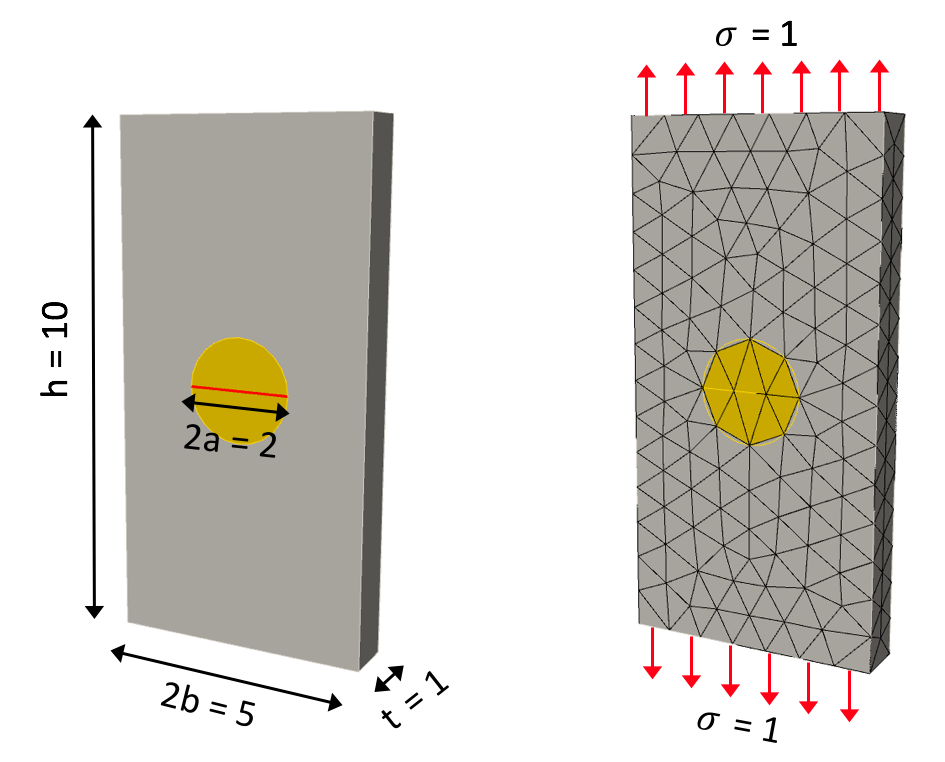
\includegraphics[width=0.5\linewidth]{Figures/plate_load_mesh.png}
	\caption{Finite plate with a horizontal crack. a) Dimensions of the specimen. b) Finite element mesh and applied stress}
	\label{fig:plate_load_mesh}
\end{figure}
The goal is to calculate the Mode I stress intensity factor $ K_I $ and compare the results to the following analytical solution \citep{rooke1976compendium} for infinite plate:
\begin{equation}\label{eq:frac_analytical}
K_t=\sigma \sqrt{\pi a} \left[  \frac{1 - \frac{a}{2b} + 0.326 (\frac{a}{b})^2 }{\sqrt{1-\frac{a}{b}}}  \right]
\end{equation}
where $\sigma $ is the applied stress. Dimensions of the specimen are presented in Figure \ref{fig:plate_load_mesh} along with the finite element model consisting of 1384 tetrahedral elements. In addition to the lading shown above, displacement constraints at three vertices of the plate are applied, to prevent rigid body motions. Young's modulus $E$ and Poisson's ratio $\nu$ are $1000$ and $0.3$, respectively. 
Hierarchical approximation basis functions enable to use the elements with variable, non-uniform orders of approximation. Hence, the influence of local and global p-refinement is investigated. The numerical analyses were taken using the same mesh, but repeated for the 1-6th order of approximations with local p-refinements up to the total order of 7, since this is the current limitation of used quadrature rule. The Mode I stress intensity factor ($K_I$) can be calculated directly from the output material forces using the following relationship: 
\begin{equation}
K_I = \sqrt{GE}
\end{equation}
Figure \ref{fig:plate_conv_no_sing} shows the deformed shape of the plate for the 2nd order of approximation. From the graph, it is evident that for the same coarse mesh and number of nodes the solution can improve drastically when the order of approximation is increased. It is worth to note the well known pathological nature of the 1st order solution, which has a much higher error due to shear locking. The minimum achieved error is $0.6\%$ for all the cases with an order of approximation set to 7. Therefore, it can be observed that the same level of accuracy can be accomplished when using a low order of global approximation with only local p-refinement as with high order on the entire mesh. Moreover, by looking at the number of degrees of freedom, it is clear that using higher order elements locally can give the same accuracy at a much lower cost of computation time since the global matrix has a much lower size.
\begin{figure}
	\centering
	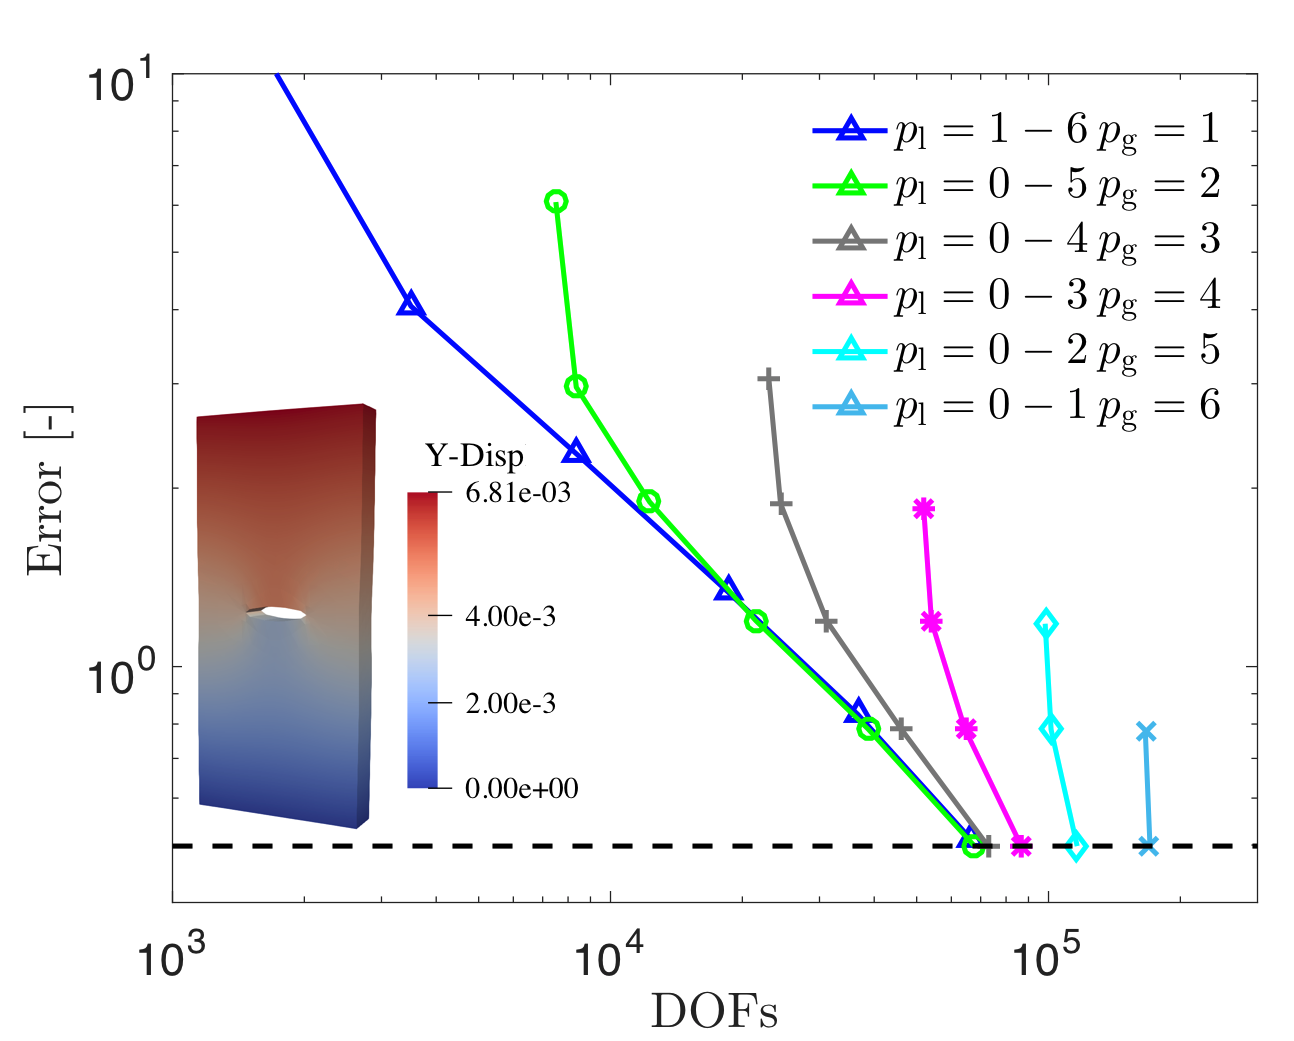
\includegraphics[width=0.7\linewidth]{Figures/graphs/plate_conv_no_sing.png}
	\caption{Convergence plot for stress intensity factor $K_I$ Error (\%) versus no. of DOF (log10) and deformed shape of the plate (bottom left).}
	\label{fig:plate_conv_no_sing}
\end{figure}
\textcolor{red}{Should I put more emphasis on this part of the work?}
\subsubsection{Quarter point elements} %should that be in appendix?
\begin{figure}
	\centering
	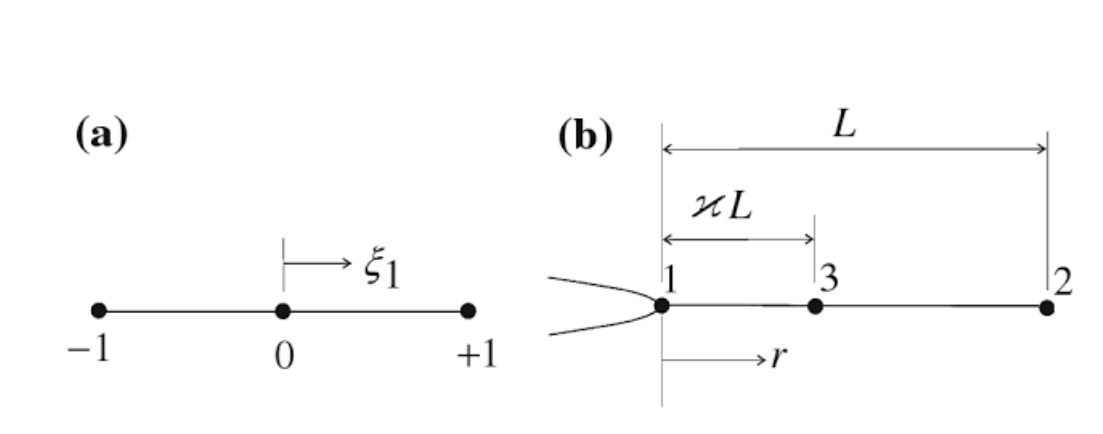
\includegraphics[width=0.7\linewidth]{Figures/1D-quarter.png}
	\caption{One-dimensional quarter-point element: a) natural coordinates, b) local Cartesian coordinates}
	\label{fig:1d-quarter}
\end{figure}
The use of finite element method to analyse fracture problems is complicated for many reasons. One of them is stress field singularity which exists at the crack tip.
Conventional finite elements are interpolated by polynomials which are not able to reproduce the infinite stress. In the mid-1970s, two independent contributors \citep{barsoum1976use,henshell1975crack} showed that the singularity at the crack tip can be modelled by placing the mid-node near the tip or front at the quarter-point position. This results in a nonlinear mapping between natural (isoparametric) and local coordinates $\xi \rightarrow x$ which produces the square root singularity. Stress and strain fields are dependent on the radial function of the crack tip, reaching infinity as $ r \rightarrow 0$. \\
This section briefly describes the reproduction of the square root singularity in quarter-point one-dimensional finite elements. 
\begin{figure}
	\centering
	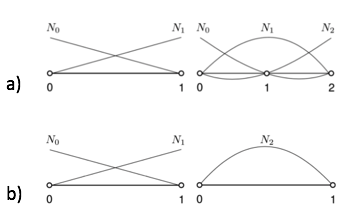
\includegraphics[width=0.5\linewidth]{Figures/shape_funcs.png}
	\caption{a) Node oriented shape functions of a 1D element. b) Hierarchical shape functions of a 1D element}
	\label{fig:shape_funcs}
\end{figure}
\subsubsection{Standard shape functions} 
The principle of quarter-point element can be straightforwardly introduced by using simple one-dimensional element as presented in Figure \ref{fig:1d-quarter} \citep{kuna2013finite}.
Let the demonstrated element be a quarter-point type at the crack tip, the distance between three nodes 1,3 and 2 is given by the coordinate $r$. The position of the middle node 3 is controlled by the parameter $\kappa$. The quadratic 1D displacement function of this element is: 
\begin{equation}\label{eq:crack_disp_func}
\begin{aligned}
&u(\xi) = \sum_{a=1}^3 N_a (\xi) u^{(a)} = \frac{1}{2} \xi (\xi - 1)u^{(1)} + (1 - \xi^2)u^{(3)} + \frac{1}{2} \xi (\xi + 1)u^{(2)} =\\
& u^{(3)} + \frac{1}{2}(u^{(2)} - u^{(1)})\xi + \left[ \frac{1}{2} (u^{(1)} + u^{(2)}) - u^{(3)} \right] \xi^2 
\end{aligned}
\end{equation}
Note that equation above is ordered by powers of $\xi$ - element natural coordinate. In the classical isoparametric formulation, the same interpolation functions are also used for the coordinates, i.e. as well for the radius $r$ with the nodal values $r^{(1)} = 0$, $r^{(3)} = \kappa L$, $r^{(2)} = L$:
\begin{equation}\label{eq:crack_radius_dep}
r(\xi) = \sum_{a=1}^3 N_a (\xi) r^{(a)} = \kappa L + \frac{1}{2} L \xi  + \left(  \frac{1}{2} - \kappa \right) L \xi^2.
\end{equation}
From Equation (\ref{eq:crack_radius_dep}) above it can be easily derived that for $ \kappa=1/4$, the radius $r(\xi(-1)) = 0$, providing the following relations:
\begin{equation}
r= \frac{L}{4}(1+\xi)^2 \quad \rightarrow \quad \xi = 2 \sqrt{\frac{r}{L}} -1,
\end{equation}
which substituted into Equation (\ref{eq:crack_disp_func}) renders the desired radial dependence of the displacements $u$ and strains $\epsilon$:
\begin{equation*}
u(r) = u^{(1)} + \left( -3u^{(1)} - u^{(2)} +4u^{(3)} \right) \sqrt{\frac{r}{L}} + 2 \left( u^{(1)} + u^{(2)} -2 u^{(3)} \right) \frac{r}{L}
\end{equation*}
\begin{equation}
\epsilon(r) = \frac{\partial u}{ \partial r} = + \left( - \frac{3}{2}u^{(1)} - \frac{1}{2}u^{(2)} +2u^{(3)} \right) \frac{1}{\sqrt{Lr}} + 2 \left( u^{(1)} + u^{(2)} -2 u^{(3)} \right) \frac{1}{L}
\end{equation}
The displacement function contains now a constant (rigid body motion) and linear function also a $\sqrt r$ term, which reproduces the displacement field at the crack tip. The strain in the quarter-point element possess of the square root $\frac{1}{\sqrt r}$ singularity.
\subsubsection{Hierarchical shape functions}
In hierarchical shape functions \citep{Ainsworth2003} no extra nodes are added for functions of order higher than the first one (see Figure \ref{fig:shape_funcs}). The hierarchical shape functions' values for an arbitrary high-order shape function are created in a hierarchical algorithm. This feature makes greatly simplifies the p- and hp- adaptivity implementation. In contrast to standard shape functions, a hierarchical counterpart of Equation~(\ref{eq:crack_disp_func}) can be written simply as:
\begin{equation}
u(\xi) = \sum_{a=1}^3 N_a (\xi) u^{(a)} = (1 -\xi)u^{(1)} + \xi(1 - \xi)u^{(3)}\gamma + \xi u^{(2)}
\end{equation}
Since there is no middle node, rewriting the above equation in terms of the radius $r$ takes the form:
\begin{equation}
r(\xi) = \sum_{a=1}^3 N_a (\xi) r^{(a)} = \xi L + \xi(1-\xi)  L  \gamma
\end{equation}
Solving the above quadratic equation for coefficient $\gamma$ gives the value of $-1$, providing relation:
\begin{equation}
r= \xi L - \xi(1-\xi)L \quad \rightarrow \quad \xi = \sqrt{\frac{r}{L}},
\end{equation}
which yields the following radial dependence for displacements and strains:
\begin{equation*}
u(r) = u^{(1)} + \left( -u^{(1)} + u^{(2)} - u^{(3)} \right) \sqrt \frac{r}{L} - u^{(3)} \frac{r}{L}
\end{equation*}
\begin{equation}
\epsilon(r) = \frac{\partial u}{\partial r} = \left( u^{(1)}  + u^{(2)} - u^{(3)}  \right) \frac{1}{2} \sqrt \frac{L}{r} + u^{(3)} \frac{1}{L}
\end{equation}
Further, emerging equations have the necessary terms to reproduce rigid body motion and pass the patch tests, as well as the desired $1 / \sqrt r$ term.
This should enable the elements adjacent to the crack front to reproduce strain singularity resulting in a more accurate finite element solution \citep{nejati2015use}. The influence of the similar procedure with tetrahedral elements will is tested in the following section.
\subsubsection{Convergence with quarter-point elements}
In this section results of the convergence upon p-refinement will be presented with the same problem as demonstrated in Section \ref{sec:plate_section}. This time, however, quarter-point tetrahedral elements were applied around the crack front.
\begin{figure}[h!]
	\centering
	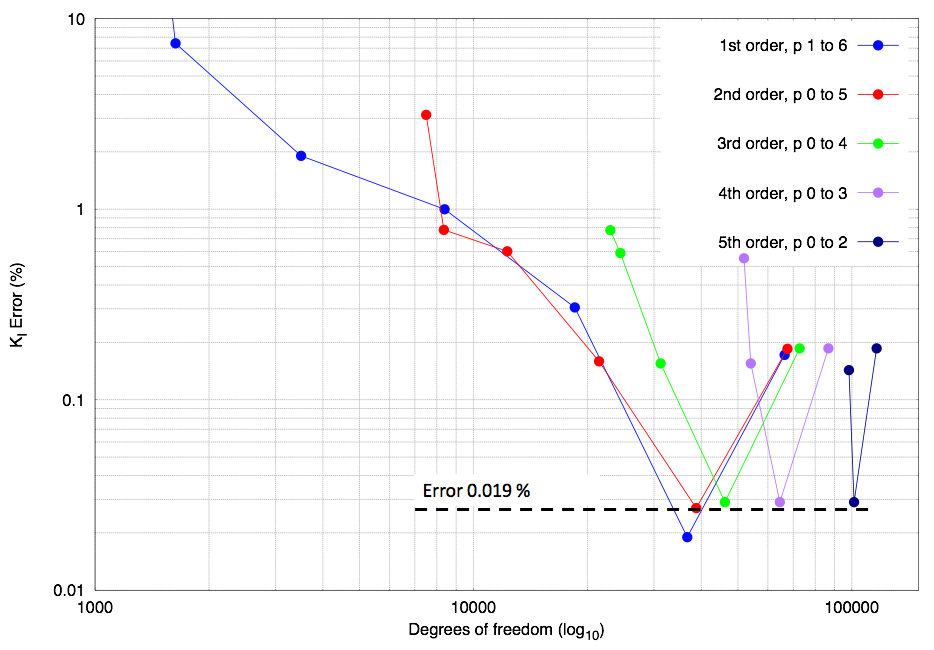
\includegraphics[width=0.7\linewidth]{Figures/graphs/plate_conv_singularity.png}
	\caption{Convergence plot for stress intensity factor $K_I$ Error (\%) versus no. of DOF (log10). It is evident that using quarter-point element enhances convergence rate.}
	\label{fig:plate_conv_singularity}
\end{figure}
Based on the results in Figure \ref{fig:plate_conv_singularity}, it is evident that using quarter-point elements improves the convergence rate to the analytical solution significantly. Introducing the singularity at the crack tip elements lowered the error by an order of magnitude, down to 0.02\%. However, it can be seen from the plot in Figure~\ref{fig:plate_conv_singularity} that for each case, just after reaching the minimum error, it starts increasing up to a certain value. This suggests that the solution cannot be further improved beyond that point only by enhancing the order of approximation. Possibly, by refining the mesh and changing model dimensions (since an analytical solution is for infinite plate), the error could be decreased even more. Nevertheless, such accuracy is redundant for engineering purposes. \\ %#overkill
%The critical thickness is that which causes the specimen to be dominated by a state of plane strain, as opposed to plane stress. The stress in the through-thickness z direction must become zero at the sides of the specimen since no traction is applied there, and in a thin specimen the stress will not have room to rise to appreciable values within the material. The strain in the z direction is not zero, of course, and the specimen will experience a Poisson contraction given by εz = ν(σx + σy). But when the specimen is thicker, material near the center will be unable to contract laterally due to the constraint of adjacent material. Now the z-direction strain is zero, so a tensile stress will arise as the material tries to contract but is prevented from doing so. 
Overall, these results indicate that it is of great benefit to use quarter-points elements, since they improve the accuracy of the solution with no extra cost, the difference in execution time for the analysis with and without their inclusion was negligible. 
\subsubsection{Validation of material forces in the heterogeneous body}
So far this paper has focused on cracks in homogeneous bodies. The following sections will discuss the influence of including inhomogeneities into the domain. Considering the same problem of the finite plate with horizontal crack, as in the previous analyses, a density field $\mathbf{\rho}(x,y,z) = 0.125y + 1$ is approximated directly onto integration (Gauss) points of each tetrahedral element, by using MLS method, demonstrated in Section \ref{sec:mwls}. Once again, stretching the specimen introduces some material forces at the crack tip and also on the entire domain due to inhomogeneity. Since the stress intensity factor loses its meaning in the case of heterogeneous bodies, how to correctly validate those forces remains an open question. To the best of the authors' knowledge, the current state of literature lacks in numerical methods to verify the results of material forces or stress intensity factors for heterogeneous solids other than functionally graded materials \citep{kim2002finite}. \\
It was decided that a straightforward verification can be performed by using simple numerical differentiation method like centered Finite Difference Method (FDM). Following Griffith's work \citep{Griffith163}, the release energy rate for crack growth can be calculated as the change in elastic strain energy per unit area of crack growth, i.e.
\begin{equation}
\mathbf G = \frac{\partial \psi}{\partial a}
\end{equation}
where $\psi$ is the elastic energy of the system, and $a$ is the crack length. Moving on, this derivative can be calculated by aforementioned FDM as follows:
\begin{equation}
 \frac{\partial \psi}{\partial a} = \lim_{\Delta a \to 0} \frac{\psi(a + \Delta a) - \psi(a -\Delta a)}{2\Delta a}
\end{equation}
where the elastic strain energies $\psi(a \pm \Delta a)$ can by obtained simply by running two additional analyses of the finite plate with horizontal cracks of lengths: ($a + \Delta a$) and ($a - \Delta a$), where $\Delta a$ is a very small value. Next, knowing the resulting release energy with the crack length of $a$, an relative error can be calculated. 26 sets of three analyses (for different p-refinements) have been performed in order to determine the error in the release energy. The results are presented in Figure \ref{fig:covergencefdm}.
\begin{figure}
	\centering
	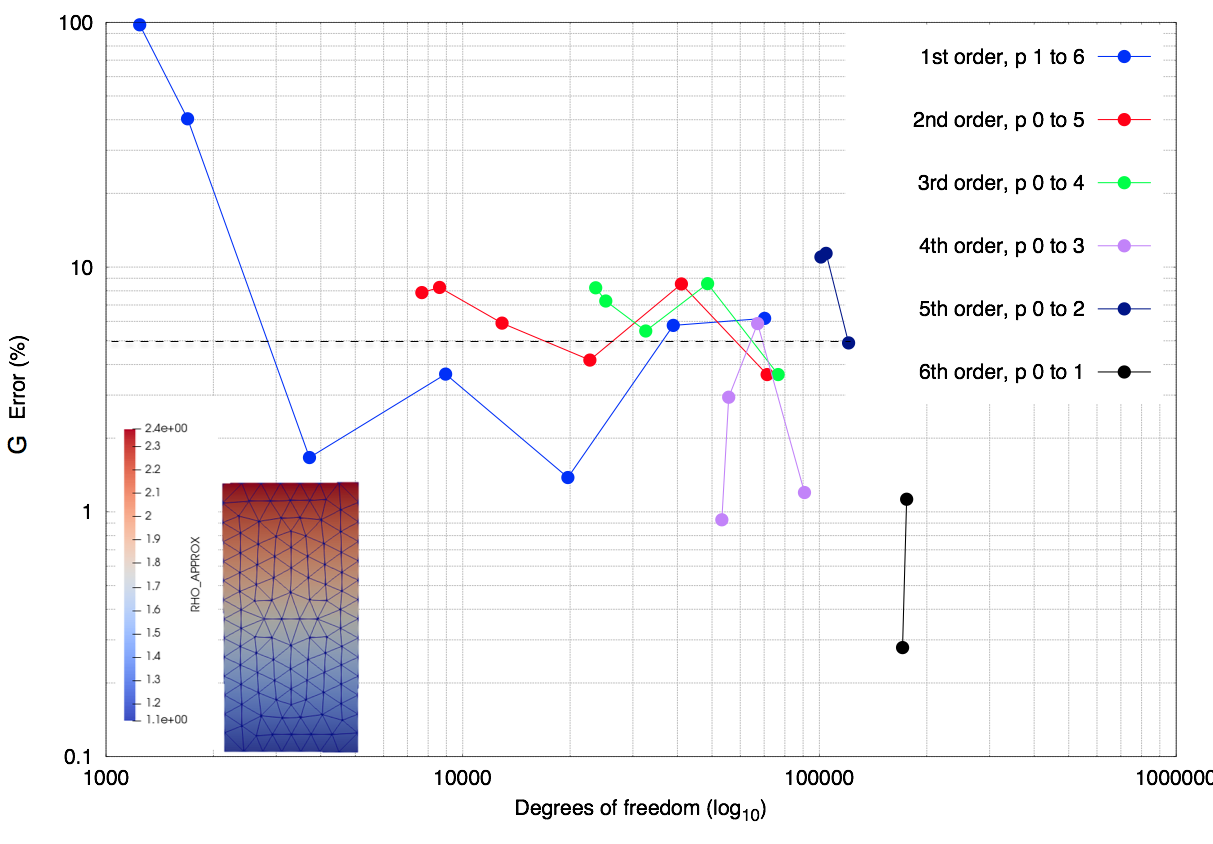
\includegraphics[width=0.7\linewidth]{Figures/graphs/covergence_FDM.png}
	\caption{Convergence of error in release energy rate from Finite Difference Method. Density distribution (bottom left).}
	\label{fig:covergencefdm}
\end{figure}
It is apparent from this plot that for most of the refinements the error in release energy is less than 5\%, which is a well known capacity of FDM.  %% REFERENCE?
Therefore, it can be deduced that the presented implementation allows for estimation of release energy for heterogeneous domains with a satisfactory level of accuracy.
\subsubsection{Release energy rate for metacarpal bone from CT}
This numerical example considers the same bone as presented in Section \ref{sec:numerical_examples:bone_adap}. The generated mesh with an initial crack is shown in Figure~\ref{fig:bone_ct_mesh_cut} and consists of 6069 tetrahedral elements. The notch is situated at the origin of the most common location of lateral condyle fracture \citep{jacklin2012frequency}. The numerical analyses were undertaken using three meshes (6069, 10032, 21189) and repeated for 1st, 2nd and 3rd-order of local p-refinement at the crack tip. Boundary conditions and material parameters remain the same as in Table \ref{tab:parameters_mc3}. Using a $ \mathrm {K_2 HPO_4  }$ calibration phantom, gray scale values from CT are converted to bone mineral density using five tubes with reference densities. The mechanical material properties were mapped onto the integration points of the metacarpal mesh using the MLS method described earlier. Applying load onto the bone surface introduces some material forces in the entire domain, with the highest values at the singularity i.e notch tip. Resulting nodal material forces are illustrated in Figure \ref{fig:crackfrontforce}. The direction of the vectors also indicates the direction of crack propagation.
%When these forces, attain the critical value, crack growth is spontaneous and catastrophic.  
The values of numerically predicted maximal nodal release energy rates in Mode I (crack opening) for subsequent meshes are plotted in Figure \ref{fig:max_g1_convergece}. It can be seen that with increasing order of approximation material forces converge.
\begin{figure}
	\centering
	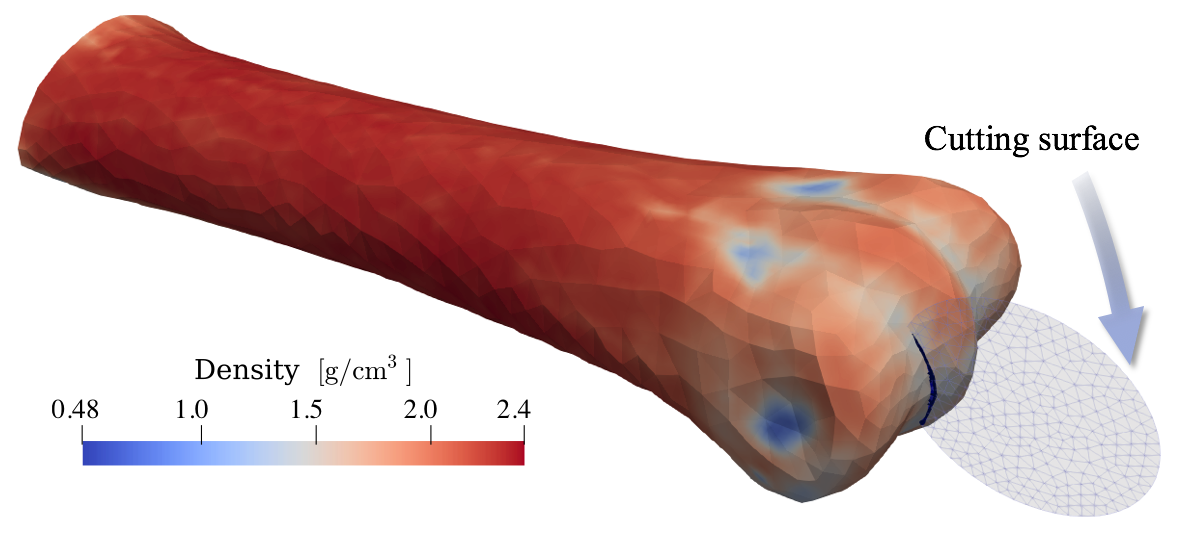
\includegraphics[width=0.5\linewidth]{Figures/bone_ct_mesh_cut.png}
	\caption{Bone geometry with mapped density from CT by using MLS. In order to calculate the material forces, an initial crack is introduced by cutting the mesh with a circular surface. The cutting algorithm is not limited to planar cracks. }
	\label{fig:bone_ct_mesh_cut}
\end{figure}

\begin{figure}
	\centering
	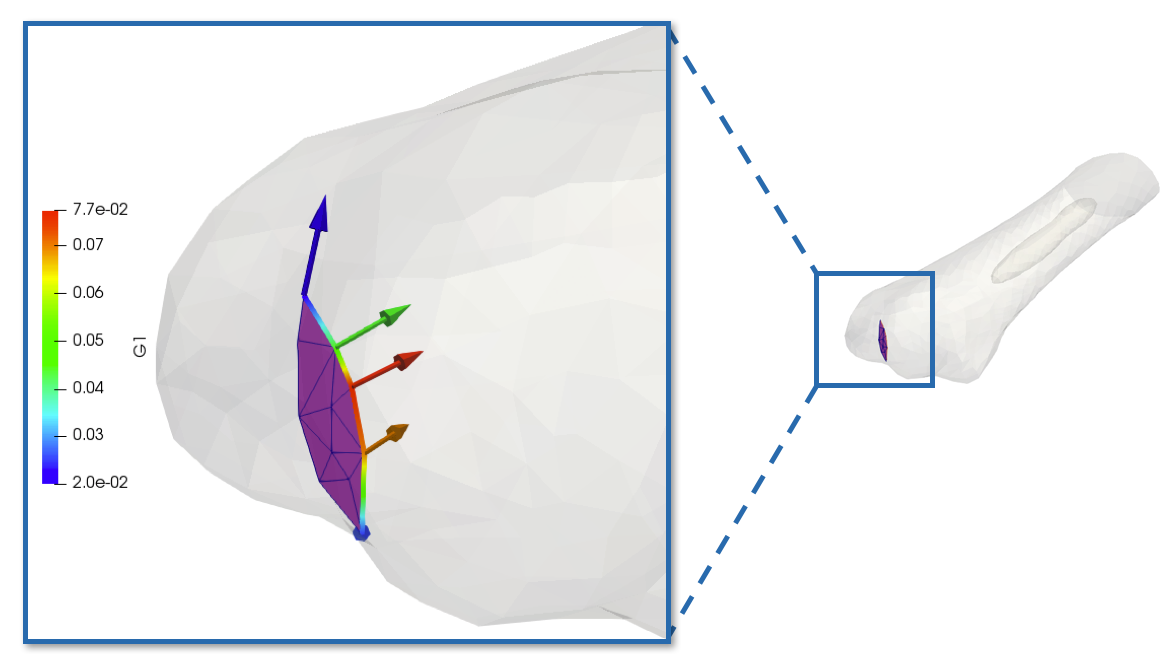
\includegraphics[width=0.9\linewidth]{Figures/crack_front_force.png}
	\caption{Crack surface and vectors of material (crack driving) forces at the front.}
	\label{fig:crackfrontforce}
\end{figure}

\begin{figure}
	\centering
	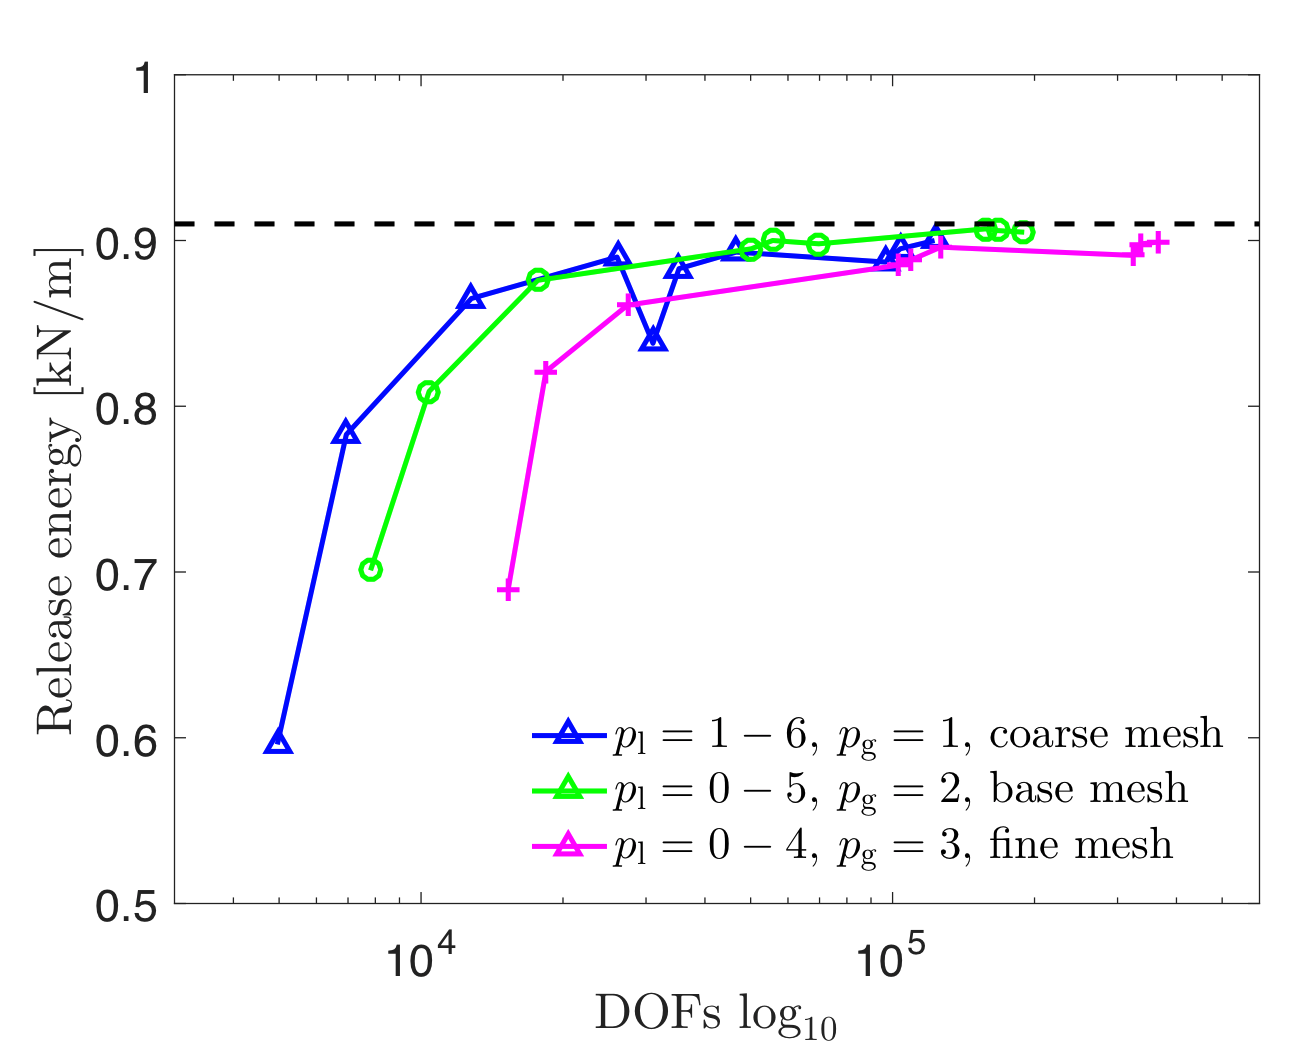
\includegraphics[width=0.7\linewidth]{Figures/graphs/max_g1_convergece.png}
	\caption{Convergence plot of maximum material force in Mode-I versus no of DOF (log10) for subsequent discretisations and p-refinements. Results are rather mesh independent and converge to the value for release energy of approximately $ G_I = 0.9 \, \mathrm{kJ} / \mathrm{m}^2$. }
	\label{fig:max_g1_convergece}
\end{figure}
Crack extension occurs when the energy release rate $G$ equals the material's resistance to crack extension. Assuming that bone's resistance is 2.0 $\mathrm{ kJ/m^2}$ ) \citep{gasser2007numerical} it can be estimated that this particular metacarpal can sustain loading of approximately 2.2 times greater before fracture starts to propagate. 
\subsubsection{Release energy rate for remodelled bone}
The numerical example described in this section presents an application of the developed framework to estimate the crack propensity of the equine metacarpal bone at different phases of adaptation during training. The same geometry and boundary conditions as in the previous example are used here. However, this time, densities from bone adaptation (Section \ref{sec:numerical_examples:bone_adap}) are mapped on a mesh consisting of 6069 elements as demonstrated in Figure \ref{fig:frackmeshcutting}. 
\begin{figure}
	\centering
	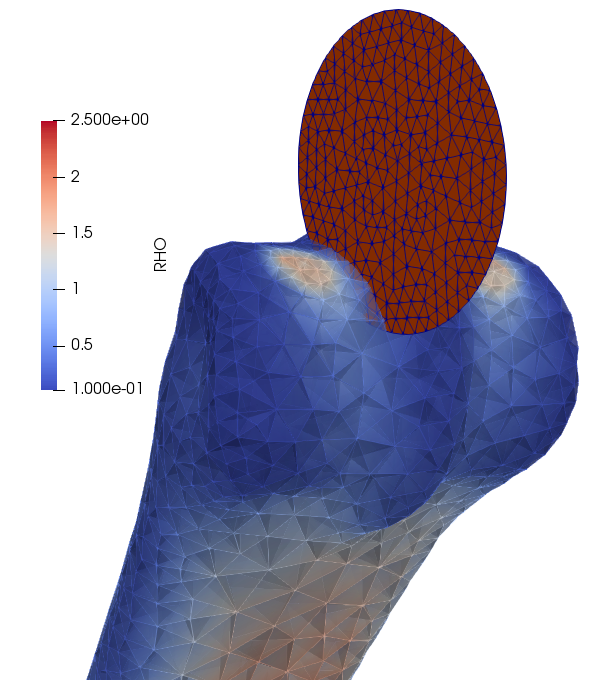
\includegraphics[width=0.4\linewidth]{Figures/frack_mesh_cutting.png}
	\caption{Cut in the mesh of the remodelled 3rd metacarpal bone. The resulting density from the bone adaptation analysis is approximated directly onto integration points of the new model by using MLS method described earlier in Section~\ref{sec:mwls}. }
	\label{fig:frackmeshcutting}
\end{figure}
The resulting energy rate at different points in time of bone adaptation are illustrated in Figure \ref{fig:crackmc3release} for three different local p-refinements. The difference between analysis with increased order at the crack tip is very small. 
\begin{figure}
	\centering
	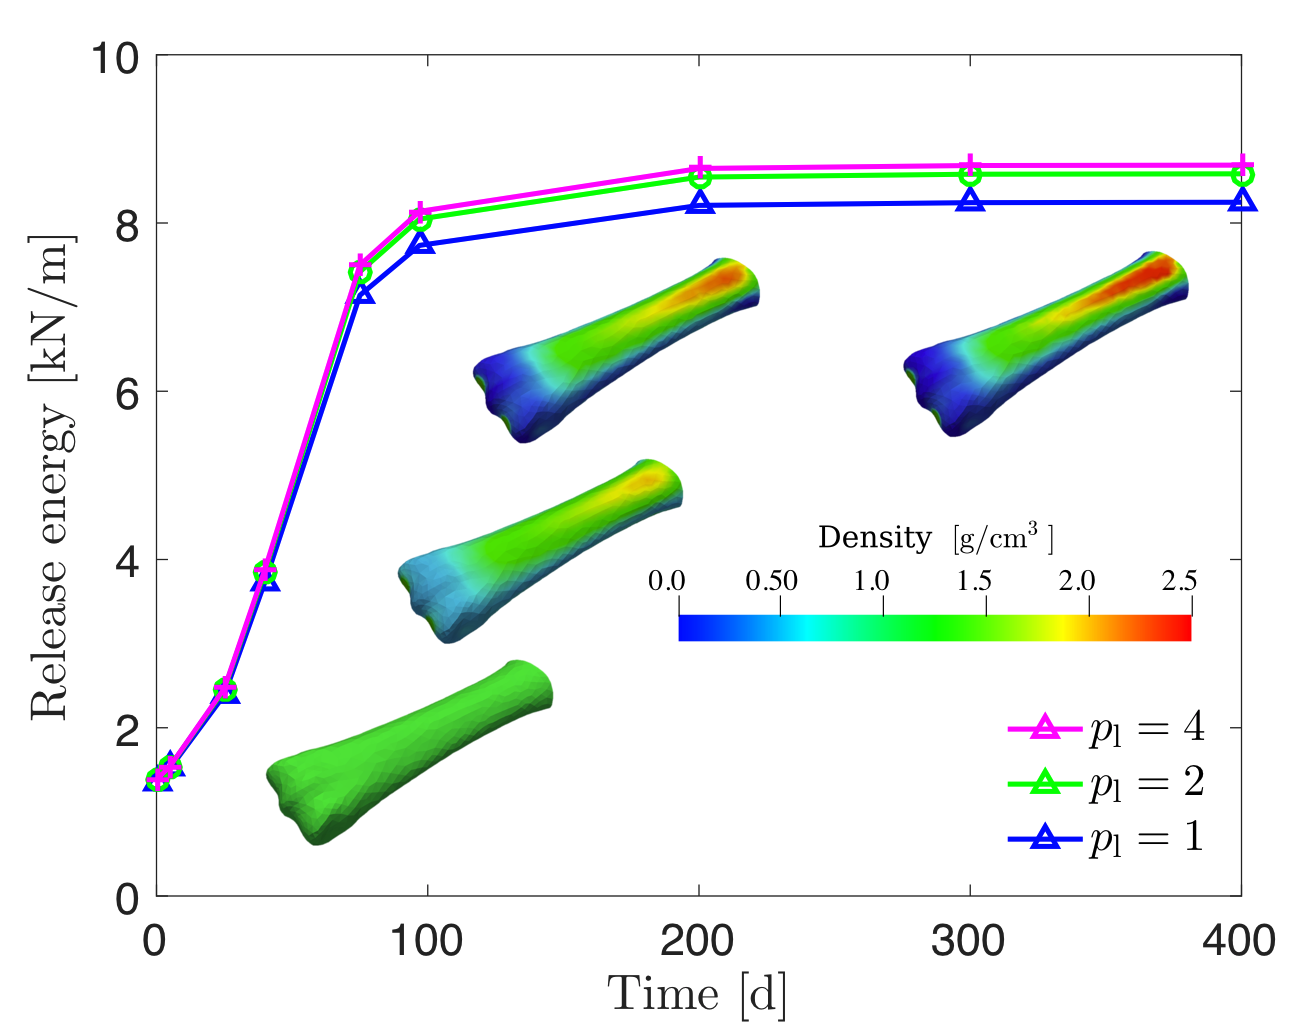
\includegraphics[width=1\linewidth]{Figures/graphs/crack_mc3_release.png}
	\caption{Material forces for remodelled bones for three local p-refinements. (nodal configurational forces)}
	\label{fig:crackmc3release}
\end{figure}
The numerical outcomes clearly capture the general trend of increasing release energy rate over time for racehorses' bones. It can be seen that by introducing a notch in the resorption zone, where no loading is applied, the material force attains larger values. This indicates that over time the presented bone becomes more prone to fracture in the specific region. 


%SIMPLY: energy release per unit length of a crack advancement has to be equal energy consumption for the creation of the new surface in the circuital conditions and its equal to %material parameter - fracture energy. Griffith theory
%$-\frac{\partial \psi}{\partial a} = \frac{\partial S}{\partial a} = \mathcal\mathbf G_c$

\section{Discussion}
Development of a 3D Finite Element model for biological applications is a very complicated process. Unlike that in typical engineering research subjects, there is still very little knowledge of the material properties. Another issue is a proper definition of the boundary conditions. Constraints are mostly explicit when analysing engineering objects such as concrete beams or steel frames under different loading conditions. However, in a living body it is challenging to accurately define loads. Model geometry suffers from inaccuracies in scanning as well as segmentation process. A~possible number of errors increase at each stage of creating such models since there is high uncertainty about obtained data \citep{campoli2014effects}. Available information is usually subject-specific or gathered for a relatively small population of subjects and cannot be generalised. Subsequently, even if one manages to overcome the aforementioned obstacles, there is a need for validation of such models, which will also have to deal with similar difficulties. Over the years, many frameworks have been developed to quantify such uncertainty levels, which might greatly increase the credibility of computational models \citep{wille2016uncertainty}. CT scanning on living horses limbs is still too cumbersome to be used as a standard diagnostic tool, as to best authors' knowledge there is a limited number of facilities that can perform CT scanning for horses without the necessity for anaesthesia. Nevertheless, this study can bring new insight in the area of catastrophic injuries in order to improve the welfare of the thoroughbred racehorse. %The successful application of developed framework would enable the introduction of interventions for veterinary practitioners, such as suggestions for training regimes based on known risk factors for lateral condylar fractures that could reduce the probability of fracture in racehorses. \\
In summary, the goals of this study were (i) implement bone remodelling algorithm to predict density levels in response to high-intensity training for racehorses (ii) to incorporate an efficient and accurate mapping strategy to represent heterogeneous bone material properties for hierarchical finite element models (iii) to assess the potential of linear fracture mechanics in evaluating bones' propensity to failure. Despite certain limitations, it was demonstrated that the implemented open systems thermodynamics framework allows for simulating of a natural behaviour of hard biological tissues. The proposed computational method may have a great potential to identify the risk of fracture related to changes in bone mineral density. Understanding the effects of changing release energy in response to bone remodelling can help developing training regimes that reduces the liability of fatal injury. Furthermore, the model uses very few parameters which can be experimentally determined in a practical manner increasing the attractiveness of this approach.\\ 
Application of a bell function to enforce bounds on density levels in the constitutive model did not provide rigid constrains for density levels, but merely slowed down the convergence to the biological equilibrium process. Nevertheless, it may still become useful, when one tries to fit the model parameters into the actual density data form CT scanning in defined periods of time. One could also constrain density bounds by introducing and calibrating mass influx to the balance of mass equation \citep{sharma2013adaptive}. Nonetheless, bones in the living organisms are never fully load adapted \citep{christen2014bone}. Therefore, achieving a biological equilibrium that results in unrealistic levels of density should never take place in a real case scenario. \\
This contribution also investigated the application of a meshless MLS method in approximating the density data on FE models. Validation of analytical field mapped on a simple mesh and comparison with LS method on mapping data from CT scanning was conducted and proved that MLS can be a suitable technique for the approximation of density field, even with strong gradients. Nevertheless, the accuracy of the presented approach still has to be validated experimentally, for example, in the prediction of strains in the loaded bone specimen.  \\
A novel method in quantifying bone fracture propensity was presented. By scanning the bone, running the bone adaptation simulation and subsequently introducing a notch in the geometry at particular time steps, it can be observed from the values of material forces how the bone loading impacts the resistance to fracture. That can be potentially a very useful tool in diagnostic of fractures and eventually prevention of catastrophic failures. Moreover, that code was developed keeping in mind scalability and robustness. Entire framework can be executed on parallel computer system in order to fit in an efficient patient-specific modelling routine that can handle many patients within a practical time window. \\
Numerical examples demonstrated the accuracy of the proposed framework. Convergence has been validated for all examples, in particular, the use of quarter point elements was shown to improve the convergence of calculated release energy rates. 
\subsection{Limitations and future work}
The methods presented in this paper had several important limitations. Considerably more work has to be done to determine loading on the bone, since using simplified input results in unrealistically low densities in non load-bearing regions. As has been proven previously, multiple load cases can be critical in modelling bone adaptation \citep{geraldes2016consideration}. In the future, the forces will be obtained by using gait data and musculoskeletal analysis \citep{Delp2007} combined with FEM mortar contact formulation in MoFEM \citep{athanasiadis2018mortar}. Another method to predict realistic loading is to solve an~inverse problem to bone remodelling. Promising results have been reported in that field by using machine learning methods like Neural Networks \citep{campoli2012computational}. The current linear fracture mechanics approach does not take into account nonlinear cohesive mechanisms like collagen fiber bridging at the crack tip \citep{yang2006fracture}. Therefore, the calculated release energy with presented approach might be overestimated. More research is also required to calibrate material parameters, in particular those regarding constitutive relations for bone remodelling. 


%Overall, the presented examples of density evolution, at this point are not sufficient to make any practical conclusions about the remodelling of the metacarpal bones. \\


%Calculation of release energy rate does not give any insights into quantitative strength of the bones' structure. Future implantation on an implicit crack propagation for heterogeneous bodies will allow to trace a full dissipative loading path. The process of determining detailed musculoskeletal loads using kinematic data and external forces is called inverse dynamic analysis

%Another limitation of the study is that only one load case is considered. 
%However, it is important to note that while simulating bone functional adaptation a detailed knowledge of the actual loading situation is elementary. By assuming that all three cases occur simultaneously in some loading conditions forces could balance each other.

%The model is not yet calibrated and validated against patient data, however, it provides valuable insight to the bone remodelling behaviour for equine metacarpal and is capable of qualitatively comparing different loading.

%bone remodelling is not purely load-driven. Possible causes for this could be that also other mechanisms, for example, calcium homeostasis, influence normal bone remodelling and thus bone is never fully load adapted. as suggested in \citep{christen2014bone}. The authors of previously mentioned publication also suggests that approximately 50\% of the bone structure might be determined by mechanical loading.


%No previous study has investigated release energy of brittle fracture in heterogeneous bodies like bones. 
%In the future we might use a micro CT scanning as ot was shown that it is currently the most accurate method to estimate bone strength. 
%We are hoping that when we refine the model we could confirm that bone remodelling may increase the propensity to cracks and find potential practical applications in the fracture prevention.
% this research can be easily translated into human applications 
%Presented framework could be also combined with other risk factors \citep{georgopoulos2017risk} which should improve the clinical assessment of fracture risk
%The correlation between bone adaptation, high intense training and stress fractures is still poorly understood. The promising results of this study offer a novel framework to simulate  changes in the bone structure as a result of loading and quantify the risk of fatal injury. 
%In conclusion, this study has shown that fracture resistance in the equine metacarpal bone can be numerically quantified. 
%Understanding the effects of changing release energy in response to bone remodelling will help in the development of training regimes that reduces the risk of fatal injury in racehorses
%This approach might become especially handy to analyse whether a discovered crack in the equine bone is liable to propagate under certain loading conditions. 
%model with the capability to simulate the bone density growth and resorption processes due to mechanical stimuli
%A reduction in this specific type of fracture would have a significant global impact on the number of Thoroughb redracehorses subjected to euthanasia as a result of in jury incurred duringracing
%has a massive welfare and economic impact on horse racing

%A better understanding of the influence of race training on subchondral bone remodelling is essential to understanding the pathophysiology of subchondral bone injury.

%Therefore, the development of computational tools with the capability to estimate bone adaptation when prosthetic devices are used has a remarkable importance, since these processes may contribute to implant success or failure. In this scenario, the finite-element method (FEM) has been playing a key role, being used to study and evaluate the mechanical behaviour of prosthetic devices

%The flexibility of the hierarchic finite element is fully utilised, which permits the use of arbitrary order of approximation leading to accurate results for relatively coarse meshes. The developed computational framework is implemented in our group's FE software, MoFEM (Mesh-Oriented Finite Element Method). \\

%Moreover, the application of the study proposes a computational assessment tool for veterinary specialists, focused on the simulation of a healthy femur and a femur with an implanted prosthesis submitted to loads.

%The main objective advocated in this contribution is the setting up of a modelling framework relying on the thermodynamics of irreversible processes




\newpage
\bibliographystyle{abbrv}
\bibliography{bibfile}
\end{document}